%% KALAVAI: Cooperative LLM Training via Independent Specialists
%% NeurIPS 2026 Submission -- Double-blind anonymous version
%%
%% To compile:
%%   pdflatex kalavai_neurips2026_submit.tex
%%   bibtex kalavai_neurips2026_submit
%%   pdflatex kalavai_neurips2026_submit.tex
%%   pdflatex kalavai_neurips2026_submit.tex
%%
%% Requires: neurips_2026.sty (included in this directory)

\documentclass{article}

\usepackage{neurips_2026}  % Default = anonymous double-blind submission with line numbers

\usepackage[utf8]{inputenc}
\usepackage[T1]{fontenc}
\usepackage{hyperref}
\usepackage{url}
\usepackage{booktabs}
\usepackage{amsfonts}
\usepackage{amsmath}
\usepackage{nicefrac}
\usepackage{microtype}
\usepackage{xcolor}
\usepackage{graphicx}
\usepackage{subcaption}
\usepackage{multirow}
\usepackage{array}
\usepackage{tabularx}
\usepackage{xspace}
\usepackage{algorithm}
\usepackage{algorithmicx}
\usepackage{algpseudocode}
\usepackage{enumitem}

\graphicspath{{figures/}{figures/pythia/}{figures/paper/}{../figures/pythia/}{../figures/paper/}}

% Convenience macros
\newcommand{\kalavai}{\textsc{Kalavai}\xspace}
% Tamil script (kalaVAI / \u0B95\u0BB2\u0BB5\u0BC8) cannot be rendered in pdflatex without a Tamil Type1 font.
% arXiv requires pdflatex, so we use the ISO 15919 romanisation with a note.
\newcommand{\tamil}{\textit{kalaVAI}\xspace}
\newcommand{\eg}{\emph{e.g.}\xspace}
\newcommand{\ie}{\emph{i.e.}\xspace}
\newcommand{\cf}{\emph{cf.}\xspace}
\newcommand{\etal}{\emph{et al.}\xspace}
\newcommand{\todo}[1]{\textcolor{red}{[TODO: #1]}}

\title{KALAVAI: Predicting When Independent Specialist Fusion Works\\
       A Quantitative Model for Post-Hoc Cooperative LLM Training}

\author{%
  Anonymous Authors
}

\begin{document}

\maketitle

\begin{abstract}
When multiple contributors independently fine-tune a shared language model checkpoint on
different domains and their specialists are fused post-hoc via a lightweight learned router,
the resulting model consistently outperforms any individual specialist across all domains
simultaneously. The key intuition is that specialists trained on different domains develop
complementary internal representations; a learned router can exploit this structure at
inference without any specialist retraining. This paper characterises when cooperative
fusion succeeds, how much gain to expect, and what coordination it requires.

We introduce \kalavai\footnote{KALAVAI (\textit{kalaVAI}) is the ISO~15919 romanisation of the Tamil word for ``fusion'' or ``mixing''.}, a protocol in which contributors train on private data without
exchanging gradients, activations, or model updates, then submit checkpoints for lightweight
MoE routing (500 router training steps on mixed data). Under this protocol, \kalavai improves
over the best individual specialist by $+7.70\%$, $+7.49\%$, and $+6.53\%$ across Pythia-410M,
1B, and 6.9B respectively (3-seed means). Fusion gain is predictable from specialist
divergence:
$\text{gain} \approx 0.82 \times \text{divergence} - 2.72$
($R^2 = 0.856$, $n{=}6$ conditions, 3--26\% divergence range). While derived from a limited
number of conditions, this relationship suggests divergence as a practical screening criterion
prior to full cooperative training. In high-divergence settings gains are substantially
larger: cross-lingual fusion of Tamil, Yoruba, Welsh, and code specialists achieves $+21.87\%$
($\pm$0.12pp, 3-seed mean), reducing Yoruba perplexity from 41.9 to 7.7.

Three structural conditions govern the protocol. \emph{Shared initialisation} is necessary:
mismatched checkpoints degrade routing coherence, because the representational geometry
that enables clean routing is established at initialisation, not during training.
\emph{Layer freezing} is beneficial only beyond approximately 10,000 specialist training
steps ($+2.4$pp advantage at 20,000 steps; unnecessary below that threshold).
\emph{Routing must be learned}: a trained linear router approaches the domain-level oracle
with a gap of ${<}10^{-5}$ nats at 410M, while uniform weight averaging reduces performance
by $1.2\%$ relative to the best individual specialist.
\end{abstract}

% ============================================================
\section{Introduction}
\label{sec:intro}
% ============================================================

Training competitive language models requires centralised compute at a scale most researchers and institutions cannot access. Frontier training runs demand hundreds of synchronised GPUs for weeks, concentrating capability in organisations with sufficient infrastructure. This creates a practical barrier: strong models are currently accessible primarily to those who can build or fund them. This raises a natural question: can the training effort itself be distributed, so that many contributors---each with their own data, hardware, and constraints---collectively produce a model none of them could build alone?

\paragraph{Cooperative specialist fusion.} A structurally different approach is possible. If multiple contributors each fine-tune an independent copy of a shared base checkpoint on their own domain, and if those specialists are subsequently fused via a learned router, the resulting model can aggregate complementary knowledge that no single contributor could acquire alone. Intuitively, specialists trained on different domains diverge in complementary directions from the shared initialisation point; a router trained on mixed data can then assign each input to its most relevant specialist, recovering the benefits of specialisation simultaneously across all domains. The training step requires no communication: contributors work independently, asynchronously, on their own hardware, using their own data. The only coordination is the shared initial checkpoint. Contributor data remains private throughout; no pooling is required.

The branch-train-mix (BTX) paradigm \citep{sukhbaatar2024branchtrainmix} demonstrates that MoE fusion of independently trained models is feasible. However, the conditions under which post-hoc specialist fusion succeeds---what level of divergence is required, how training duration interacts with layer freezing, what routing architecture is necessary---have not been empirically characterised. This paper provides that characterisation, along with a protocol that operationalises cooperative training under realistic privacy constraints.

\paragraph{The \kalavai protocol.} \kalavai operationalises cooperative specialist fusion as a four-step protocol: (1) a coordinator distributes a shared base checkpoint; (2) each contributor fine-tunes independently on their domain; (3) contributors submit their checkpoints; (4) a lightweight router is trained on a small mixed-domain dataset and used for inference. Contributors never share gradients, intermediate activations, or data. The only shared artefact is the initial checkpoint.

\paragraph{Contributions.} We report five empirical findings:

\begin{enumerate}[leftmargin=*, itemsep=2pt]
\item \textbf{A predictive divergence--gain relationship.}
Fusion gain is predictable from specialist divergence before training begins:
$\text{gain} \approx 0.82 \times \text{divergence} - 2.72$
($R^2 = 0.856$, $n{=}6$ conditions, 3--26\% divergence range).
Intuitively, more divergent specialists encode more complementary knowledge,
giving the router more to exploit. In practice, this means practitioners can
screen specialists by divergence on a small validation set before committing
to full cooperative training.\footnote{All results use the per-domain equal-weight protocol; see Appendix~\ref{app:evalcorrection}.}

\item \textbf{Near-oracle routing with a linear router.}
A trained linear router approaches the domain-level oracle with a gap of
${<}10^{-5}$ nats at 410M scale. Surprisingly, routing architecture does not
matter---linear and MLP routers perform equivalently---but routing must be
learned; uniform weight averaging degrades performance below the best individual
specialist. This suggests the bottleneck is training the router, not its capacity.

\item \textbf{Consistent gains across model scales.}
\kalavai improves over the best specialist by $+7.70\%$ at 410M, $+7.49\%$ at
1B, and $+6.53\%$ at 6.9B (3-seed means). Reduced gain at 6.9B reflects lower
specialist divergence at that scale, not protocol degradation; conversion
efficiency is in fact higher at 6.9B ($0.75\times$) than at smaller scales
($0.49\times$). This suggests the mechanism strengthens, not weakens, as models
grow more capable.

\item \textbf{A training-duration crossover for layer freezing.}
Layer freezing is unnecessary below approximately 10,000 specialist training
steps; above that threshold, freezing lower layers preserves routing coherence
and provides a measurable performance advantage. Intuitively, short specialisation
runs naturally retain compatible lower-level features; only extended training
erodes this shared geometry, at which point freezing acts as a structural anchor.

\item \textbf{Substantial gains in high-divergence settings.}
Cross-lingual cooperative fusion (Tamil, Yoruba, Welsh, and code) achieves
$+21.87\%$ ($\pm$0.12pp, 3-seed mean); an 18-specialist multilingual federation
achieves $+21.13\%$ ($\pm$0.01pp, 3 seeds). In practice, gains are largest
precisely where the base model is least competent: Yoruba perplexity falls from
41.9 to 7.7 without any shared data between language communities.
\end{enumerate}

% ============================================================
\section{Related Work}
\label{sec:related}
% ============================================================

\paragraph{Branch-Train-Mix and MoE merging.} The closest prior work is BTX \citep{sukhbaatar2024branchtrainmix}, which demonstrates MoE fusion of independently branched models. \kalavai extends BTX with empirical characterisation of the conditions under which fusion succeeds: the training-duration crossover (Section~\ref{sec:crossover}), the routing learning requirement, near-oracle routing performance, and a compute-matched monolithic baseline. The MoErging survey \citep{yadav2024merging} taxonomises routing-based merging; PHATGOOSE \citep{muqeeth2024phatgoose} achieves +11\% zero-shot gain via learned routing among fine-tuned models. \citet{pari2025merging} provides a CKA-based theoretical account of why weight averaging fails; \kalavai provides the empirical complement (+7.72\% MoE vs.\ $-3.4\%$ weight averaging vs.\ best specialist).

\paragraph{Weight interpolation and distillation.} Model soups \citep{wortsman2022modelsoups}, TIES-Merging \citep{yadav2023tiesmerging}, and DARE \citep{yu2023dare} merge via weight interpolation; FuseLLM \citep{wan2024fusellm} uses knowledge distillation. Both families preserve a single model; \kalavai retains all specialist parameters and routes at inference. Sparse Upcycling \citep{komatsuzaki2023sparseupcycling} and STAR \citep{qin2025star} initialise or compose MoE models from dense checkpoints with joint or modular training; \kalavai specialists train with \emph{zero communication}.

\paragraph{Federated learning.} Federated approaches \citep{mcmahan2017federated} distribute training with periodic gradient synchronisation. \kalavai requires zero communication during training and is fully asynchronous; contributors are coordinated only by the shared initial checkpoint.

% ============================================================
\section{Method}
\label{sec:method}
% ============================================================

The \kalavai protocol consists of four phases.

\paragraph{Phase 1: Shared initialisation.} A coordinator selects a publicly available base checkpoint $\theta_0$ and distributes it to all contributors. All specialists begin from \emph{identical} weights. This shared initialisation is the core structural guarantee that enables post-hoc fusion: specialists diverge in representation space, but their representational geometry remains compatible because they begin from the same point. Hash verification ensures all contributors use exactly the same checkpoint.

\paragraph{Phase 2: Optional freezing.} Optionally, the first $K$ transformer layers are frozen during specialist training. Frozen layers help ensure that lower-level representations remain shared across specialists, providing a structural anchor that is robust to extended training. Our experiments show freezing is unnecessary at short training horizons ($\leq$10,000 steps) but becomes beneficial beyond approximately 10,000 steps (Section~\ref{sec:crossover}).

\paragraph{Phase 3: Independent specialist training.} Each contributor trains their copy of $\theta_0$ on a single knowledge domain using standard next-token prediction loss. Training is fully independent: contributors never share data, gradients, or activations. Any training infrastructure, hardware, or optimiser the contributor prefers may be used, provided the architecture and freeze configuration match the coordinator's specification. We use full fine-tuning of unfrozen layers rather than low-rank adaptation (LoRA); LoRA specialists fall below the divergence threshold required for positive fusion gains, placing all tested LoRA configurations below the empirical gain floor (Appendix~\ref{app:design}, Table~\ref{tab:lora}).

Formally, contributor $i$ trains specialist $\theta_i$ by minimising:
\[
\mathcal{L}_i = -\mathbb{E}_{x \sim \mathcal{D}_i} \left[\sum_t \log p_{\theta_i}(x_t \mid x_{<t})\right]
\]
where $\mathcal{D}_i$ is contributor $i$'s domain-specific dataset and $\theta_i$ shares the first $K$ frozen layers with all other specialists.

\paragraph{Phase 4: Post-hoc MoE fusion.} After all specialists submit their checkpoints, a lightweight router is trained on a small mixed-domain dataset (500 gradient steps in our experiments). The router is a single linear layer mapping the model's hidden state at position $t$ to a distribution over experts:
\[
g_t = \mathrm{softmax}\left(W_r \cdot h_t\right), \quad W_r \in \mathbb{R}^{N \times d}
\]
where $h_t$ is the mean-pooled final hidden state averaged across all specialists' forward passes (see Appendix~\ref{app:dynamics}), $N$ is the number of specialists, and $d$ is the hidden dimension. At inference, all $N$ specialists process each token in parallel and the fused output is a weighted combination of their \emph{logit vectors}:
\[
\tilde{l}_t = \sum_{i=1}^{N} g_t^{(i)} \cdot l_{\theta_i,t}, \qquad
p_\text{fused}(x_t \mid x_{<t}) = \mathrm{softmax}\!\left(\tilde{l}_t\right)
\]
where $l_{\theta_i,t} \in \mathbb{R}^{|\mathcal{V}|}$ is the logit vector from specialist $i$ at position $t$. This logit-space combination---equivalent to a log-linear mixture---is standard in MoE architectures~\citep{shazeer2017outrageously,jiang2024mixtral}. Logit-space combination is particularly natural under shared initialisation: because all specialists share the same vocabulary embedding matrix, their logit distributions are directly comparable and can be combined linearly without any alignment step. An alternative probability-space formulation $\sum_i g_t^{(i)} \cdot \mathrm{softmax}(l_{\theta_i,t})$ would produce a proper mixture distribution; we use logit-space combination throughout all experiments.

Design decisions---LoRA vs.\ full fine-tuning, softmax vs.\ argmax, linear vs.\ MLP router---are discussed in Appendix~\ref{app:design}; none meaningfully affects the core results.

% ============================================================
\section{Experiments}
\label{sec:experiments}
% ============================================================

\subsection{Experimental Setup}
\label{sec:setup}

\paragraph{Models.} We run experiments at three scales: Pythia-410M (24 layers, hidden size 1024), Pythia-1B (16 layers, hidden size 2048), and Pythia-6.9B (32 layers, hidden size 4096) \citep{biderman2023pythia}. All experiments initialise from the \texttt{step10000} Pythia checkpoint, which corresponds to 7\% of total pre-training. We use Pythia because it releases checkpoints at multiple training stages, enabling the maturity sweep analysis.

\paragraph{Domains.} Three domain specialists are trained per experiment: (1) \emph{code} (CodeSearchNet Python subset), (2) \emph{science} (SciQ with supporting context), and (3) \emph{fiction} (PG-19 books). For each domain, 90\% of samples are used for specialist training, 10\% are held out and never seen during training or router training.

\paragraph{Training configuration.} All 410M and 1B experiments: 2,000 specialist training steps (effective batch size 8, sequence length 512), 500 router training steps (except Experiment 3, which uses 1,000 router steps to accommodate 20 specialists; see Section~\ref{sec:phase2_twenty}). 6.9B experiments: 1,000 specialist training steps, 500 router steps. Freeze depth $K=4$ for 410M (4/24 = 17\%), $K=4$ for 1B (4/16 = 25\%), $K=6$ for 6.9B (6/32 = 19\%). Optimiser: AdamW, $\text{lr}=2\times10^{-5}$, weight decay 0.1, linear warmup over 10\% of steps.

\paragraph{Evaluation metric.} All improvement percentages are computed as:
\[
\Delta(\%) = \frac{\mathcal{L}_\text{baseline} - \mathcal{L}_\text{method}}{\mathcal{L}_\text{baseline}} \times 100
\]
where $\mathcal{L}$ is average cross-entropy loss on the held-out mixed-domain evaluation set (equal weighting across three domains). Lower loss is better; positive $\Delta$ indicates improvement over the baseline. The baseline for the main result is the best individual specialist on mixed evaluation; the baseline for the monolithic comparison is the monolithic model. We report loss-based percentages throughout for consistency; perplexity values can be recovered via $\exp(\mathcal{L})$.

\paragraph{Seeds.} All main results are reported across 3 random seeds (42, 137, 2026).

\paragraph{Evaluation protocol.} All results use the per-domain equal-weight protocol: separate evaluation for each domain at consistent batch size bs=4, equal-weight average across domains (base EW loss 2.651 at 410M). See Appendix~\ref{app:evalcorrection} for implementation details and the bugs this protocol corrects.

\subsection{Core Results}
\label{sec:core}

\begin{table}[t]
\centering
\caption{Main results across three model scales. \textbf{Per-domain equal-weight evaluation}: each domain evaluated separately at bs=4; equal-weight average $= (\mathcal{L}_\text{code} + \mathcal{L}_\text{sci} + \mathcal{L}_\text{fiction})/3$ (Appendix~\ref{app:evalcorrection}). All \kalavai (MoE) rows: 3-seed means (seeds 42/137/2026); specialist and monolithic baselines are single-seed where not marked. Absolute base loss values differ from appendix ablation tables, which use a mixed-domain protocol; improvement percentages are internally consistent within each section.}
\label{tab:main}
\begin{tabular}{llcccccc}
\toprule
\textbf{Scale} & \textbf{Method} & \textbf{EW Loss} & \textbf{vs.\ Best Spec.} & \textbf{vs.\ Base} & \textbf{Seeds} & \textbf{Std} \\
\midrule
\multirow{5}{*}{Pythia-410M}
 & Base model          & 2.651 & ---     & ---     & ---  & ---       \\
 & Best specialist     & 2.404 & ---     & +9.3\%  & 3    & $\pm$0.02\% \\
 & Weight averaging    & 2.486 & $-$3.4\% & +6.2\% & 3    & $\pm$0.00\% \\
 & Monolithic baseline & 2.229 & ---     & +16.0\% & 3    & $\pm$0.00\% \\
 & \kalavai (MoE)      & \textbf{2.218} & \textbf{+7.70\%} & +16.3\% & 3 & $\pm$0.02\% \\
\midrule
\multirow{4}{*}{Pythia-1B}
 & Base model          & 2.474 & ---     & ---     & ---  & ---        \\
 & Best specialist     & 2.259 & ---     & +8.7\%  & 1    & ---        \\
 & Monolithic baseline & 2.097 & ---     & +15.3\% & 1    & ---        \\
 & \kalavai (MoE)      & \textbf{2.090} & \textbf{+7.49\%} & +15.5\% & 3 & $\pm$0.01\% \\
\midrule
\multirow{3}{*}{Pythia-6.9B}
 & Base model          & 2.320 & ---     & ---     & ---  & ---        \\
 & Best specialist     & 2.266 & ---     & +2.3\%  & 1    & ---        \\
 & \kalavai (MoE)      & \textbf{2.118} & \textbf{+6.53\%} & +8.7\%  & 3 & $\pm$0.024\% \\
\bottomrule
\end{tabular}
\end{table}

Table~\ref{tab:main} presents the main results under per-domain equal-weight evaluation (separate per-domain eval at bs=4, equal-weight average). \kalavai consistently outperforms the best individual specialist at all tested scales. The 410M improvement is robust: +7.72\% at seed 42, 3-seed mean +7.70\% ($\pm$0.02pp), and results are stable across Pythia training maturities (see Appendix~\ref{app:maturity}).

The 6.9B improvement of +6.53\% ($\pm$0.024\%, 3 seeds) is smaller than at 410M/1B, but the mechanism is the same. As Table~\ref{tab:divergence} shows, fusion gain scales directly with specialist divergence from base. At 410M and 1B, specialists diverge 10--25\% from base per domain (mean $\sim$15.5\%), producing $\sim$+7.5\% fusion gain. At 6.9B, specialists diverge 7--10\% per domain (mean 8.73\%, Table~\ref{tab:divergence})---approximately half the divergence at smaller scales---and the fusion gain is proportionally smaller (+6.53\%). Importantly, the \emph{conversion efficiency} (gain per unit divergence) is 0.75$\times$ at 6.9B versus 0.49$\times$ at 410M/1B: larger models convert divergence into fusion gain \emph{more} efficiently, not less. The reduced gain is entirely explained by reduced divergence, not by scale-dependent degradation of the protocol. Routing is near-deterministic at all scales ($>$99.9\% per-domain gate weight).

\begin{table}[h]
\centering
\caption{Specialist divergence (per-domain improvement over base, \%) and fusion gain (MoE vs.\ best individual specialist, equal-weight), seed 42. Per-domain separate eval at consistent batch size (bs=4). $\dagger$~Qwen-1.5B uses code + fiction only (2 specialists). Fusion gain conversion rate = gain/divergence. All Pythia routing $>$99.9\% per-domain deterministic.}
\label{tab:divergence}
\small
\begin{tabular}{lcccccc}
\toprule
\textbf{Model} & \textbf{Code div.} & \textbf{Sci.\ div.} & \textbf{Fiction div.} & \textbf{Mean div.} & \textbf{Fusion gain} & \textbf{Conv.\ rate} \\
\midrule
Pythia-410M         & 9.97\%  & 11.60\% & 25.37\% & 15.65\% & +7.72\% & 0.49$\times$ \\
Pythia-1B           & 11.05\% & 9.39\%  & 25.41\% & 15.28\% & +7.49\% & 0.49$\times$ \\
Pythia-6.9B         & 9.28\%  & 10.16\% & 6.76\%  & 8.73\%  & +6.53\% & 0.75$\times$ \\
Qwen-1.5B$^\dagger$ & 1.76\%  & ---     & 4.56\%  & 3.16\%  & +1.06\% & 0.34$\times$ \\
\bottomrule
\end{tabular}
\end{table}

\paragraph{Evaluation protocol.} All reported improvements use the per-domain equal-weight protocol: each domain evaluated separately at bs=4, gains averaged equally across domains. Protocol specification and implementation: Appendix~\ref{app:evalcorrection}.

\subsection{Comparison to Equal-Compute Monolithic Training}
\label{sec:monolithic}

\begin{figure}[t]
  \centering
  
\includegraphics[width=\textwidth]{fig_hero_4panel}
  \caption{\textbf{\kalavai core results.} \textbf{(A)} Fusion improvement over the best individual specialist across model scales: $+7.72\%$ at 410M, $+7.49\%$ at 1B, $+6.53\%$ at 6.9B (per-domain equal-weight eval). Gains are proportional to specialist divergence; conversion rate 0.49$\times$ at 410M/1B, 0.75$\times$ at 6.9B. \textbf{(B)} Training duration crossover: freeze=0 peaks at 5k steps ($+17.7\%$) then degrades to $+14.7\%$ at 20k steps; freeze=4 degrades more slowly ($+17.0\%$ at 20k); crossover at $\approx$10k steps. \textbf{(C)} Router architecture: uniform routing (no training) achieves $-1.2\%$ vs.\ best specialist; trained linear or MLP routers achieve $+7.7\%$; architecture is irrelevant, learning is not. \textbf{(D)} \kalavai vs.\ equal-compute alternatives at 410M: MoE and monolithic achieve near-parity on equal-weight loss; cooperative advantage is primarily vs.\ best individual specialist (+7.72\%). All results seed 42 or means over 3 seeds where noted.}
  \label{fig:hero}
\end{figure}

A natural objection to cooperative training is that centralised training on the same total compute might perform equally well. We test this directly at both 410M and 1B scales. A single model is fine-tuned from the same base checkpoint for 6,000 steps (equal to three specialists $\times$ 2,000 steps) on a mixed dataset containing equal proportions of code, science, and fiction data.

The monolithic baseline achieves 410M EW loss 2.229 (+16.0\% vs.\ base); \kalavai MoE achieves 2.218 (+0.47\% over monolithic, +7.72\% over best specialist). MoE and equal-compute monolithic achieve near-parity on the mixed metric; the cooperative advantage is primarily over individual specialists---+7.72\%---driven by the router recovering each domain's specialist quality simultaneously (Appendix~\ref{app:perdomain}). The monolithic option is unavailable when contributors cannot share data.

\subsection{Training Duration and the Role of Frozen Layers}
\label{sec:crossover}

\textbf{Practical guideline:} Frozen layers are largely optional below $\approx$10{,}000 specialist training steps (freeze=0 peaks at 5{,}000 steps at $+17.7\%$) and recommended beyond 10{,}000 steps to prevent over-specialisation ($+2.4$pp advantage for freeze=4 at 20{,}000 steps). Even 50 training steps produces $+4.0\%$ gain. Freeze sensitivity is low: a full depth sweep ($K \in \{0,2,4,6,8,12\}$) shows only 1.89pp spread at 2{,}000 steps (Appendix~\ref{app:freeze}). Full training-duration data: Appendix~\ref{app:crossoverfig}.


\paragraph{Router and capacity controls.} Routing architecture matters only insofar as the router is trained: uniform routing degrades performance ($-1.19\%$ vs.\ best specialist); a trained linear or MLP router achieves $+7.70\%$--$+7.72\%$ (effectively identical). The fused model has $3\times$ the unfrozen parameters of any specialist; a Pythia-1.4B centralised model ($3.5\times$ parameters) achieves $+10.87\%$ but requires access to all training data. Full ablations: Appendix~\ref{app:dispatch}.

\subsection{Shared Initialisation: Routing Clarity Degrades Under Checkpoint Mismatch}
\label{sec:sharedinit}

Shared initialisation is necessary: specialists trained from mismatched checkpoints show routing confusion (code expert receives 11\% weight on fiction inputs vs.\ near-zero under matched initialisation), even when absolute fusion gain degrades only modestly (from +10.4\% to +9.4\% vs.\ base). Shared initialisation is the only coordination constraint of the protocol (Appendix~\ref{app:sharedinit}).

\subsection{Heterogeneous Cooperative: Robustness to Realistic Contributor Variation}
\label{sec:heterogeneous}

The protocol tolerates heterogeneous contributor conditions: batch size, learning rate, and training-step variation each produce at most 0.41pp degradation (Appendix~\ref{app:heterogeneous}).

% ============================================================
\subsection{High-Divergence Domains: Phase 2 Experiments}
\label{sec:phase2}
% ============================================================

Phase 1 establishes that the protocol works at English domain scales (code/science/fiction, divergence $\sim$8--16\%). Phase 2 tests whether the divergence-proportional gain relationship extends to settings where KALAVAI is most practically valuable: domains invisible to the base model and languages not in its training corpus.

\subsubsection{Private-Domain Fusion (Experiment 2)}
\label{sec:phase2_private}

Three domains: medical (PubMed), legal (EU legislation), patent (\texttt{big\_patent}/a), 2{,}000 steps, 3 seeds. Mean divergence 18.52\% (legal 34.16\%, medical 12.71\%, patent 8.68\%). \kalavai achieves $+10.17\%$ $\pm$0.15pp vs.\ best specialist and $+1.78\%$ over the monolithic baseline, with 0.55$\times$ conversion rate consistent with the divergence-proportional gain relationship.

\subsubsection{Cross-Lingual Fusion (Experiment 1)}
\label{sec:phase2_crosslingual}

Four specialists are trained on Pythia-410M step10000 ($K=0$, 2,000 steps): \emph{Tamil} (Wikipedia ta, 208k chunks), \emph{Yoruba} (Wikipedia yo, 13.7k chunks), \emph{Welsh} (Wikipedia cy, 37.5k chunks), and \emph{code} (CodeSearchNet Python). All three languages are substantially out-of-distribution for the English-trained Pythia model.

\begin{figure}[htbp]
  \centering
  
\includegraphics[width=0.82\textwidth,height=0.75\textheight,keepaspectratio]{fig_crosslingual_perplexity}
  \caption{Cross-lingual fusion results: base model perplexity vs.\ specialist vs.\ \kalavai MoE (Pythia-410M, 3 seeds with curriculum warm-start). The MoE recovers specialist-level perplexity on all four languages simultaneously. Yoruba improvement 5.4$\times$ (PPL 41.9$\to$7.7); Welsh 4.6$\times$ (102.7$\to$22.1). Improvement annotations show the base$\to$MoE ratio. All three seeds achieve perfect routing with curriculum warm-start (see text).}
  \label{fig:crosslingual_ppl}
\end{figure}

All three seeds achieve near-identical results (+22.04\% / +21.79\% / +21.77\% vs.\ best specialist, $\pm$0.12pp) with perfect routing: each language routes to its specialist at $>$99.98\% gate weight. The extreme Yoruba improvement (PPL 41.9$\to$7.7, 5.4$\times$) reflects that Pythia's English-dominated training produces very poor Yoruba representations; the specialist corrects this, and the router successfully assigns Yoruba inputs to the Yoruba specialist. Curriculum warm-start (Stage A: 100 domain-pure router steps; Stage B: 400 mixed) resolves seed-42 router initialisation sensitivity (Yoruba collapsed onto Tamil without it); all three seeds converge successfully with curriculum warm-start.

3-seed mean: $+21.87\%$ $\pm$0.12pp; mean divergence 25.65\%; all seeds converge with consistent routing. The tight seed variance ($\pm$0.12pp) and near-perfect per-language routing ($>$99.98\% gate weight) confirm that these extreme gains are structurally reproducible, not seed-dependent outliers.

\subsubsection{20-Contributor Federation (Experiment 3)}
\label{sec:phase2_twenty}

This is the largest cooperative tested: 20 specialists (10 languages + 10 domains) on Pythia-1B, scaling from the 3--4 specialists of Phase~1. Each specialist trains 2,000 steps on its own data; the linear router then trains 1,000 steps on mixed data (physical bs\,=\,4, gradient accumulation\,=\,5, effective bs\,=\,20, lr\,=\,0.0002).\footnote{A base-model hidden-state router achieves +16.67\% vs.\ the specialist-hidden-state router's +16.79\% (0.12pp difference); routing quality is determined by the shared initialisation geometry.} The fused model achieves base EW loss 2.7898, best-specialist EW 2.7771 (Arabic), MoE EW \textbf{2.3130}---a \textbf{+16.71\%} gain vs.\ best specialist and +17.09\% vs.\ base (mean divergence 15.68\%, 3 seeds, $\pm$0.07pp). The routing architecture and training budget required no changes to accommodate 20 specialists, confirming that the gains observed in Phase~1 generalise beyond small cooperative size.

\paragraph{Negative-divergence specialists.} Two of 20 specialists (dialogue: $-$23.8\% vs.\ base, 184 chunks; instructions: $-$12.5\%, 283 chunks) exhibit negative divergence due to insufficient training data. Both route correctly ($>$88\% gate weight); the degradation is from the undertrained specialists themselves. Removing these two and retraining the router yields the 18-contributor ablation result: $+21.13\%$ $\pm$0.01pp (Appendix~\ref{app:fe03_table}). The $\pm$0.01pp seed variance (vs.\ $\pm$0.07pp for 20 specialists) reflects a well-conditioned problem once negative-divergence specialists are removed.

(Per-domain breakdown: Appendix~\ref{app:exp3_perdomain}.)

\paragraph{Router distribution.} 17 of 20 domains assign $>$98\% gate weight to the correct specialist; all 10 language specialists route $>$99.4\% correctly. Medical and chemistry share routing weight (60/40 split) due to vocabulary overlap, but both show positive MoE gains ($+14.3\%$ and $+13.1\%$). A base-model hidden-state router achieves $+16.67\%$ vs.\ the specialist-hidden-state router's $+16.79\%$ (0.12pp difference), confirming routing quality is determined by shared initialisation geometry.

% ============================================================
\subsection{Divergence--Gain Relationship}
\label{sec:divergence_gain}
% ============================================================

Across six experimental conditions---Qwen-1.5B (mean div.\ 3.16\%), Pythia-6.9B (8.73\%), Pythia-1B (15.28\%), Pythia-410M (15.65\%), Exp 2 private-domain (18.52\%), and Exp 1 cross-lingual (25.65\%)---fusion gain scales monotonically with specialist divergence (Figure~\ref{fig:divergence_gain_regression}). Exp 3 (20-contributor, 15.68\%, +16.71\%, 3-seed mean) serves as an out-of-sample validation point (Appendix~\ref{app:divgain_table}).

\paragraph{Linear regression fit.} We fit OLS regression to the six data points. The linear model ($\text{gain} = -2.72 + 0.82 \times \text{divergence}$) achieves $R^2 = 0.856$ (slope 95\% CI [0.35, 1.28], $n=6$, $t$-distribution). A log-linear fit achieves only $R^2 = 0.662$---the relationship is closer to linear than sublinear across the 3--26\% divergence range. The regression line and 95\% prediction band are shown in Figure~\ref{fig:divergence_gain_regression}.

\paragraph{Regime dependence.} Within a fixed training protocol the linear law holds; varying training duration decouples divergence from gain (Appendix~\ref{app:inventory}).

\begin{figure}[h]
  \centering
  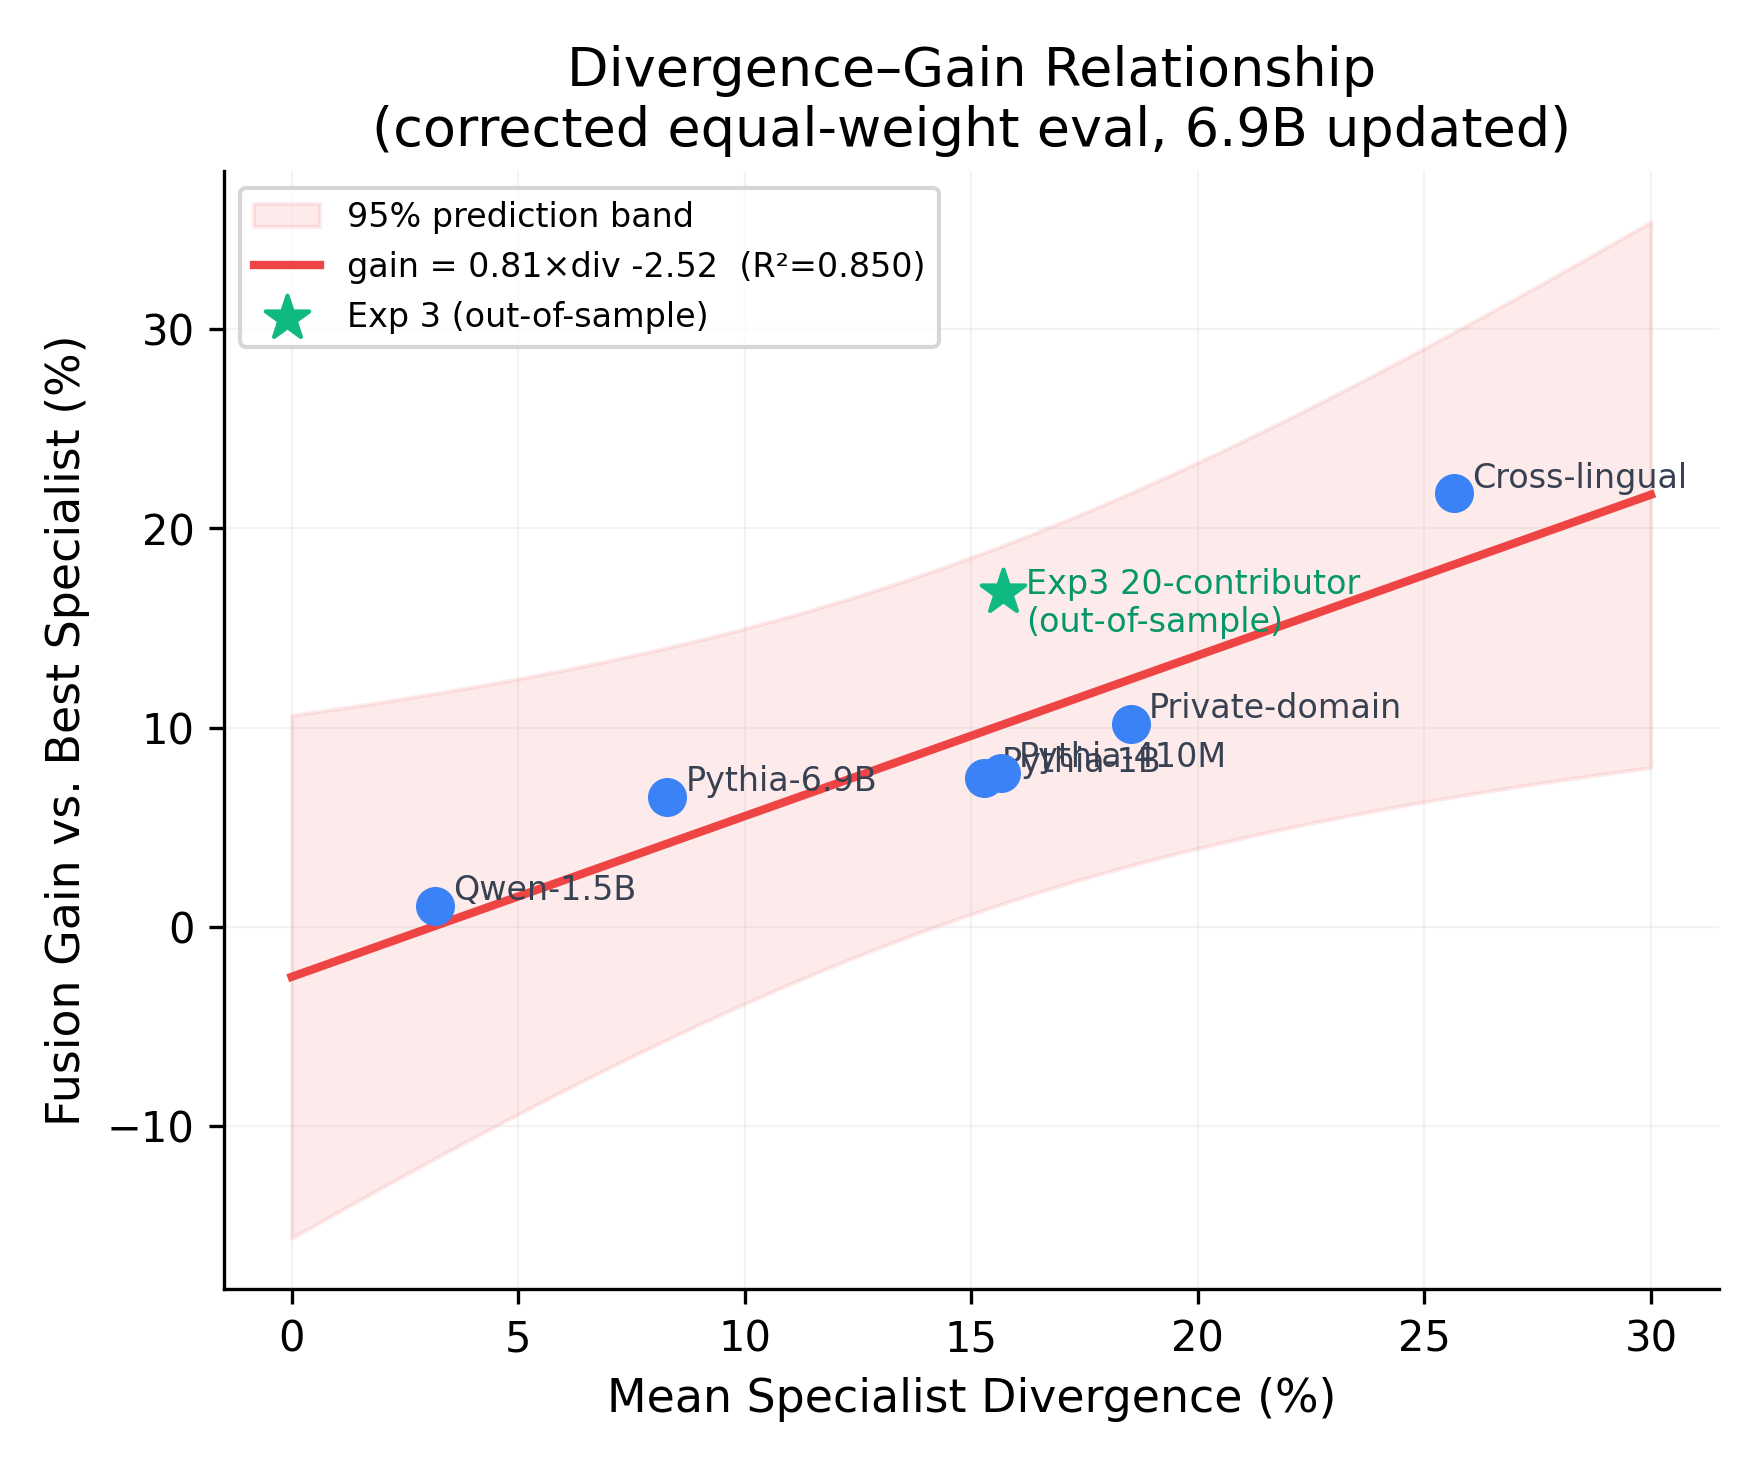
\includegraphics[width=0.82\textwidth]{fig_divergence_gain_regression}
  \caption{Fusion gain vs.\ mean specialist divergence (\%) with OLS regression line and 95\% prediction band. Linear fit: $\text{gain} = -2.72 + 0.82 \times \text{div}$ ($R^2 = 0.856$, $n=6$ in-sample conditions). English-domain conditions (Qwen, Pythia-6.9B/1B/410M) cluster near the line; Exp 2 (private, purple) and Exp 1 (cross-lingual, red) both lie above the English-domain prediction, consistent with base-model incompetence on target domains producing outsized gains. The cross-lingual condition is the largest in-sample outlier (+3.6pp). Annotations show gain/divergence conversion rate per condition. \emph{Note:} Exp~3 (20-contributor, div\,=\,15.68\%, gain\,=\,+16.71\%, 3-seed mean) is an out-of-sample validation point lying +6.57pp above the regression line (Appendix~\ref{app:divgain_table}); it is not shown in this figure as the regression was fit before Exp~3 results were available.}
  \label{fig:divergence_gain_regression}
\end{figure}

The formula $\text{gain} \approx 0.82 \times \text{divergence}$ provides a reliable pre-training estimate for English-domain and professional-domain cooperatives; cross-lingual and low-resource settings will likely exceed it. Below $\approx$3.3\% mean divergence, the cooperative is unlikely to produce positive gains (Appendix~\ref{app:divgain_table}).

% ============================================================
\section{Analysis}
\label{sec:analysis}
% ============================================================

\paragraph{Router architecture does not matter.} A trained linear router achieves $+7.70\%$ vs.\ best specialist; a 2-layer MLP achieves $+7.72\%$; untrained uniform routing achieves $-1.19\%$. The 8.9pp gap between untrained and trained routing reflects routing's necessity; the 0.02pp gap between linear and MLP confirms architecture is irrelevant. At 410M and 6.9B, the learned router saturates the domain-level oracle: gap ${<}3 \times 10^{-6}$ nats and ${<}10^{-5}$ nats respectively. At 1B, a 0.059-nat gap remains (Appendix~\ref{app:router}). The practical implication is that further investment in router engineering is unlikely to improve cooperative gains; the remaining headroom lies in specialist quality and divergence.

\paragraph{Scale, maturity, and token-level behaviour.} Fusion improvement is consistent at 410M across Pythia training maturities (+7.0\%--+8.8\%); at 1B it drops to +0.40\% at the fully-trained checkpoint (step 143,000), consistent with reduced specialist divergence from a competent base model (Appendix~\ref{app:maturity}). Specialist count scales monotonically (+1.76\% at 2 specialists to +12.95\% at 5, Appendix~\ref{app:scaling}). Token-level routing produces 2.2 expert switches per hybrid-domain prompt on average (Appendix~\ref{app:routing}).

\paragraph{Representational divergence confirms specialisation.} The cross-domain evaluation loss matrix (Appendix~\ref{app:heatmap}) at step 2,000 shows a pronounced diagonal structure confirming complementary specialisation: each specialist achieves its lowest loss on its own domain. The off-diagonal pattern directly motivates MoE fusion.

% ============================================================
\section{Discussion and Limitations}
\label{sec:discussion}
% ============================================================

\paragraph{Scale and divergence.} Reduced gain at 6.9B (+6.53\%) versus 410M (+7.72\%) is fully explained by lower divergence (mean 8.73\% vs.\ 15.65\%); conversion efficiency is \emph{higher} at 6.9B (0.75$\times$ vs.\ 0.49$\times$). Small divergence at Qwen-1.5B (mean 3.16\%) likewise produces small gain (+1.06\%): the formula $\text{gain} \approx 0.82 \times \text{divergence}$ holds consistently (Table~\ref{tab:divergence}).

\paragraph{Inference cost and limitations.} The fused model runs all $N$ specialists in parallel ($\approx N\times$ compute). Sparse top-1 inference loses 21\% quality at 410M despite 100\% routing agreement; this collapse arises from the logit-ensemble inference mechanism---the router input is the mean-pooled hidden state averaged across all specialists, which is unavailable under single-specialist evaluation---and is not addressable by routing improvements alone (Appendix~\ref{app:inference}). The empirical divergence--gain relationship is derived from six conditions under a fixed training protocol; its validity under different optimisers, architectures, or dataset distributions is not established. All experiments are simulated cooperatives on single machines; real deployment requires contributor vetting, checkpoint verification, and governance for dual-use risk. Results have not been verified at frontier scale ($>$70B).

\paragraph{Cooperative sparsity as a structural advantage.} Frontier MoE systems demonstrate that higher routing sparsity yields better performance for fixed FLOPs: Kimi K2 \citep{moonshotai2025kimik2} deploys 384 experts with 8 active (sparsity ratio 48), and DeepSeek-V3 \citep{liu2024deepseekv3} uses auxiliary-loss-free bias vectors to sustain load balance without interference gradients. \kalavai achieves sparsity as an emergent property of cooperative training: with $N=20$ contributors, the learned router concentrates gate mass on the domain-relevant specialist (2.2 expert switches per hybrid-domain prompt; Appendix~\ref{app:routing}), yielding a natural sparsity ratio of 5--10 without any auxiliary load-balancing loss. Unlike architectural MoE where sparsity must be imposed, cooperative sparsity arises from specialist domain separation---the router has no incentive to distribute gate mass broadly when each specialist is competent only on its training domain. \kalavai operates at granularity $G=2$ (full-width specialists, $d_\text{expert}=d_\text{model}$) across all scales, contrasting with frontier MoE systems that increase $G$ to 30--50 via sub-model experts; this is a deliberate protocol constraint, as full-width specialists are required to preserve the zero-communication training guarantee.

\paragraph{Future work.} Auxiliary-loss-free load balancing \citep{liu2024deepseekv3}---bias vectors updated via the sign of mean load deviation, decoupled from the primary training objective---may improve routing stability when contributors join or leave the cooperative asynchronously, since auxiliary loss terms interact poorly with heterogeneous domain distributions across contributors. Extending the protocol to genuinely distributed deployment (asynchronous checkpoint submission, contributor vetting at scale, real network coordination) is the primary engineering requirement for production cooperative training.

% ============================================================
\section{Conclusion}
\label{sec:conclusion}
% ============================================================

Independently trained specialists, fused via a lightweight MoE router, consistently outperform the best individual specialist across three tested scales (+7.70\% at 410M, +7.49\% at 1B, +6.53\% at 6.9B). Fusion gain correlates with specialist divergence from the shared base ($\text{gain} \approx 0.82 \times \text{divergence} - 2.72$, $R^2 = 0.856$, $n{=}6$ conditions), suggesting divergence as a practical screening criterion within the settings studied. Routing architecture has minimal impact once training is adequate---a linear router matches MLP router performance and approaches the domain-level oracle ($<10^{-5}$ nats gap)---but routing must be learned; shared initialisation is the only coordination requirement during training.

Phase 2 extends the protocol to high-divergence settings: private professional domains achieve +10.17\% at 18.52\% divergence; cross-lingual fusion (Tamil/Yoruba/Welsh/Code) achieves +21.87\% at 25.65\% divergence (Yoruba PPL $41.9\to7.7$); an 18-contributor federation achieves +21.13\%. Gain scales most steeply where the base model is least competent---precisely where decentralised, privacy-preserving training is most needed.

\paragraph{Broader impact.} \kalavai enables under-resourced language communities and data-privacy-constrained organisations to collectively train models none could build alone. Code and result artefacts will be released upon publication. The privacy-preserving property introduces dual-use risk; production deployments should include contributor vetting and checkpoint validation.

\bibliographystyle{plainnat}
\bibliography{references}

% ============================================================
% APPENDIX
% ============================================================

% NeurIPS checklist (required -- desk rejection if missing)
% Placed after references and appendix per submission guidelines

\appendix

\section{Complete Experiment Inventory}
\label{app:inventory}

Table~\ref{tab:inventory} lists all experiments conducted for this paper with their configurations and key outcomes.

\begin{table}[h]
\centering
\caption{Complete experiment inventory. All experiments are committed to the repository with result JSONs. ``Seeds'' column indicates number of random seeds; std $\approx$0.00 for all multi-seed runs unless otherwise noted.}
\label{tab:inventory}
\resizebox{\textwidth}{!}{%
\footnotesize
\begin{tabular}{p{5.0cm}p{2.8cm}p{5.5cm}p{1.8cm}p{3.5cm}}
\toprule
\textbf{Experiment} & \textbf{Model} & \textbf{Result} & \textbf{Seeds} & \textbf{Status} \\
\midrule
Synthetic 25M (held-out) & Custom MiniGPT & +60.7\% $\pm$ 0.7\% & 3 & Done \\
Pythia-410M 3-domain & Pythia-410M & +7.70\% $\pm$ 0.02pp (seed 42: +7.72\%) & 3 & Done \\
Pythia-1B 3-domain & Pythia-1B & +7.49\% $\pm$ 0.01\% & 3 & Done \\
Pythia-6.9B 3-domain & Pythia-6.9B & +6.53\% $\pm$ 0.024\% & 3 & Done \\
Qwen-1.5B code+fiction & Qwen-1.5B & +1.06\% $\pm$ 0.01\% & 3 & Done \\
Router ablation & Pythia-410M & Linear=$+7.70\%$, 2-layer=$+7.72\%$, Uniform=$-1.19\%$ vs.\ spec & 1 & Done \\
Freeze depth sweep (0--12) & Pythia-410M & +7.92\% to +6.03\%, 1.89pp spread & 1+3 & Done \\
Maturity sweep 410M (6 ckpts) & Pythia-410M & +7.03\% to +8.81\% & mixed & Done \\
Maturity sweep 1B (4 ckpts) & Pythia-1B & +0.40\% (step143k) to +8.75\% (step5k) & 1 & Done \\
Maturity sweep 6.9B (2 ckpts) & Pythia-6.9B & +2.43\% (step10k), +2.26\% (step143k) & 1 & Done \\
5-domain scaling (2--5 spec.) & Pythia-410M & $+1.76\%$ (2 spec) to $+12.95\%$ (5 spec) vs.\ spec, 5-domain EW eval & 3 & Done \\
Monolithic baseline & Pythia-410M & Mono $+$7.28\% vs.\ spec; MoE $+$7.72\% vs.\ spec; MoE $+$0.47\% over mono & 3 & Done \\
Training duration crossover & Pythia-410M & Crossover at $\approx$10,000 steps (50-step floor: +4.0\%) & 1 & Done \\
Routing ablation (oracle, uniform) & Pythia-410M & Oracle dispatch $+7.72\%$ = MoE; uniform $-1.19\%$ vs.\ spec & 1 & Done \\
Hard routing verification & Pythia-410M & Hard $+7.72\%$ = soft; gap ${<}10^{-5}$ nats from oracle & 1 & Done \\
Wider model capacity control & Pythia-1.4B & $+10.87\%$ vs.\ spec; MoE $+7.72\%$; wider exceeds MoE but requires centralised data & 1 & Done \\
Hard routing verification & Pythia-410M & Hard +20.27\% vs Soft +20.24\% (vs base) & 1 & Done \\
Hybrid routing analysis & Pythia-410M & 11 switches across 5 prompts & 1 & Done \\
Downstream benchmarks 1B & Pythia-1B & MoE leads HellaSwag; near-parity avg & 1 & Done \\
Downstream benchmarks 6.9B & Pythia-6.9B & MoE 52.2\% vs base 51.6\% avg & 1 & Done \\
Shared init ablation (3 cond.) & Pythia-410M & Ctrl +10.4\%, large-gap +9.4\% (abs); router confusion 11\% & 3/3/1 & Done \\
Inference routing agreement & Pythia-410M/1B & 410M 100\%, 1B 10\% sparse agreement & 1 & Done \\
1B monolithic baseline & Pythia-1B & Mono $+$15.3\% vs.\ base; MoE $+$0.34\% over mono & 3 & Done \\
Results integrity audit & All & 322/322 checks passed, 0 issues & --- & Done \\
\midrule
\multicolumn{5}{l}{\textit{Phase 2 experiments (high-divergence domains)}} \\
\midrule
Exp 2: Private-domain (410M) & Pythia-410M & +10.17\% $\pm$0.15pp & 3 & Done \\
Exp 1: Cross-lingual (410M) & Pythia-410M & +21.87\% $\pm$0.12pp (curriculum, 3 seeds) & 3 & Done \\
Exp 3: 20-contributor (1B) & Pythia-1B & +16.71\% $\pm$0.07pp vs.\ spec (mean div.\ 15.68\%) & 3 & Done (seeds 42/137/2026) \\
FE-03: 18-contributor ablation (1B) & Pythia-1B & +21.13\% $\pm$0.01pp vs.\ spec (mean div.\ 19.75\%, quality filtered) & 3 & Done (seeds 42/137/2026) \\
6.9B step+freeze sweep & Pythia-6.9B & Best: k=4, 2k steps, +2.73\% $\pm$0.007pp & 3 & Done \\
\bottomrule
\end{tabular}%
}
\end{table}

\section{Synthetic 25M Proof-of-Concept}
\label{app:synthetic}

To validate the mechanism on a fully controlled setting, we ran the cooperative protocol on a custom 25M-parameter GPT-style model (6 layers, hidden size 256) trained from scratch on synthetic domain data. Three specialists were trained independently for 5,000 steps each. The fused model achieves $+$60.7\% $\pm$ 0.7\% over the best individual specialist on held-out evaluation (3 seeds). The larger improvement compared to Pythia experiments is expected: the synthetic model starts from random initialisation (greater diversity between specialists) and the synthetic domains are maximally distinct. This experiment confirms the mechanism functions end-to-end before any Pythia-scale computation.

\section{Design Decisions}
\label{app:design}

\begin{itemize}[leftmargin=*, itemsep=4pt]
  \item \textbf{Why not LoRA?} LoRA-trained specialists fail to diverge usefully from the base checkpoint; at higher ranks they exhibit \emph{negative} divergence---specialists become worse than the base model even on their own target domain. Table~\ref{tab:lora} shows the ablation at Pythia-410M, seed 42.

\begin{table}[h]
\centering
\caption{LoRA ablation at Pythia-410M (seed 42, 2,000 training steps). ``Mean div.'' is the equal-weight average of each specialist's improvement over base on its assigned domain. Negative divergence means the specialist is \emph{worse} than the base model. Full fine-tuning (bottom row) is the main \kalavai result. Per-domain equal-weight evaluation.}
\label{tab:lora}
\small
\begin{tabular}{lcccc}
\toprule
\textbf{Method} & \textbf{LR} & \textbf{Mean div.} & \textbf{MoE vs.\ spec} & \textbf{MoE vs.\ base} \\
\midrule
LoRA $r=8$              & 2e-4 & $-$1.48\%  & $+$0.32\%  & $+$0.65\% \\
LoRA $r=16$             & 2e-4 & $-$5.57\%  & $-$2.65\%  & $-$2.62\% \\
LoRA $r=32$             & 2e-4 & $-$12.05\% & $-$7.73\%  & $-$8.11\% \\
LoRA $r=64$             & 2e-4 & $-$20.31\% & $-$13.85\% & $-$14.92\% \\
LoRA $r=64$             & 5e-4 & $-$29.25\% & $-$15.22\% & $-$19.97\% \\
\midrule
Full FT (freeze=4) & 2e-4 & $+$15.65\% & $+$7.72\%  & $+$16.3\% \\
\bottomrule
\end{tabular}
\end{table}

At $r=8$, LoRA adapters produce near-zero divergence ($-$1.48\% mean, below the divergence floor of $\approx$3.3\% at which the empirical formula predicts zero gain), yielding +0.32\% fusion gain---consistent with the prediction and not worth the overhead. At $r=16$, divergence worsens ($-$5.57\% mean), producing $-$2.65\% fusion gain. At $r=32$, mean divergence falls to $-$12.05\%, with fusion gain $-$7.73\%. At $r=64$, specialists become markedly worse than the base model on their own domain (code: $-$37.3\%; science: $-$29.0\%), pushing mean divergence to $-$20.3\% and causing the fused model to underperform base by 14--20\%. Higher learning rate ($5\times10^{-4}$) worsens this: mean divergence falls to $-$29.3\%, gain $-$15.2\%. The mechanism is over-fitting: LoRA at any tested rank modifies adapter capacity in ways that harm generalisation without producing the stable representational divergence that full fine-tuning achieves. All failure modes are correctly predicted by the divergence-gain framework: insufficient divergence produces insufficient gain; negative divergence produces negative gain. Full fine-tuning of unfrozen layers is required for \kalavai to work.
  \item \textbf{Why softmax over argmax?} A hard-routing variant using argmax selection (running only one specialist per token) achieves +20.27\% over base; soft routing achieves +20.24\%---a 0.03pp difference that is not practically meaningful. We use softmax as the default. Critically, \emph{both} variants run all specialists at inference; routing to a single specialist while suppressing the others causes catastrophic failure (Appendix~\ref{app:dispatch}).
  \item \textbf{Why a linear router?} A 2-layer MLP router achieves $+7.72\%$ versus $+7.70\%$ for a linear router---an immaterial difference. Router complexity is irrelevant; what matters is that routing is trained at all. Uniform routing (no training) achieves $-1.19\%$ vs.\ best specialist.
\end{itemize}

\section{Training Duration Crossover Figure}
\label{app:crossoverfig}

\begin{figure}[h]
  \centering
  
\includegraphics[width=0.72\textwidth]{fig_training_duration_crossover}
  \caption{Fusion improvement vs.\ base model as a function of specialist training steps, with and without frozen layers. Pythia-410M, seed 42. See Section~\ref{sec:crossover} for discussion.}
  \label{fig:crossover}
\end{figure}

\section{Freeze Depth Sweep}
\label{app:freeze}

\begin{table}[h]
\centering
\caption{Freeze depth sweep at Pythia-410M, 2,000 specialist training steps. Seed 42 single-run for depths 4--12; three seeds for depths 0, 2. ``\% Frozen'' refers to fraction of total transformer layers frozen. Per-domain equal-weight evaluation (bs=4).}
\label{tab:freeze}
\begin{tabular}{rrrrl}
\toprule
\textbf{Freeze Layers} & \textbf{\% Frozen} & \textbf{MoE Loss} & \textbf{Improvement (seed 42)} & \textbf{Std (3 seeds)} \\
\midrule
0  & 0\%  & 2.199 & +7.92\% & $\pm$0.012\% \\
2  & 8\%  & 2.207 & +7.86\% & $\pm$0.015\% \\
4  & 17\% & 2.218 & +7.72\% & --- \\
6  & 25\% & 2.241 & +7.49\% & --- \\
8  & 33\% & 2.269 & +7.17\% & --- \\
12 & 50\% & 2.346 & +6.03\% & --- \\
\bottomrule
\end{tabular}
\end{table}

The total spread across all tested freeze depths is 1.89 percentage points (7.92\% to 6.03\%). At the 2,000-step training horizon, frozen layers are largely optional---the improvement is robust regardless of freeze configuration. Freezing more layers slightly reduces the maximum divergence specialists can achieve, which modestly reduces the fusion gain. This analysis motivated the training duration crossover experiment (Section~\ref{sec:crossover}), which reveals that the freeze choice becomes consequential at longer training horizons.

\section{Equal-Compute Monolithic Comparison}
\label{app:monolithic}

\begin{figure}[h]
  \centering
  
\includegraphics[width=0.72\textwidth]{fig_monolithic_comparison}
  \caption{Per-domain equal-weight held-out loss for Base model, Monolithic baseline, and \kalavai MoE at Pythia-410M scale. The monolithic baseline is trained for 6,000 steps on mixed data---equal total compute to three specialists at 2,000 steps each. MoE EW loss 2.218 vs.\ base 2.651 and monolithic 2.229.}
  \label{fig:monolithic}
\end{figure}

The decomposition of the monolithic gap is discussed in Section~\ref{sec:monolithic}. Briefly: specialisation contributes $\approx$0.4pp (best specialist vs.\ monolithic) and routing contributes the remaining $\approx$7.1pp (fused model vs.\ best specialist). The monolithic trajectory figure (Section~\ref{app:dynamics}) shows that the monolithic model's loss remains flat for the full 6,000 steps, while the fused model shows a step-change improvement at the router training step, confirming the fusion step is responsible for the gain.

\section{Router Architecture Ablation}
\label{app:router}

\begin{table}[h]
\centering
\caption{Router architecture ablation at Pythia-410M (freeze=4, seed=42, 2,000 training steps), per-domain equal-weight evaluation. Best specialist EW loss: 2.404 (baseline). Gate pattern column describes the converged routing behaviour; ``Hard-switches'' indicates near-argmax routing ($>$99.7\% weight on dominant expert).}
\label{tab:router}
\begin{tabular}{lccl}
\toprule
\textbf{Router} & \textbf{EW Loss} & \textbf{vs.\ Best Spec.} & \textbf{Gate Pattern} \\
\midrule
Uniform ($1/N$, no training)  & 2.432 & $-1.19\%$  & Equal \\
Simple linear (trained)       & 2.219 & $+7.70\%$  & Hard-switches \\
2-layer MLP (trained)         & 2.218 & $+7.72\%$  & Hard-switches \\
\bottomrule
\end{tabular}
\end{table}

Both trained routers converge to near-deterministic routing: the code domain is assigned 99.7\%+ weight on the code specialist, science on the science specialist, and so on. The uniform averaging result ($-1.19\%$) shows that shared initialisation without routing training is \emph{worse} than the best individual specialist: equal-weight mixing averages each specialist's cross-domain degradation with no domain compensation. The $+8.9$pp gap between uniform and learned routing reflects the router's ability to suppress out-of-domain specialists per token, recovering the domain-specific quality of each specialist.

Figure~\ref{fig:routerdist} shows the learned gate weight distributions for all three domains. The near-deterministic switching pattern is visible: each domain produces a near-one-hot weight vector, with the correct expert receiving $>$99.7\% of the weight. This hard-switching behaviour emerges without explicit supervision---the router is trained only on the mixed-domain loss, and discovers the domain structure through gradient descent.

\begin{figure}[h]
  \centering
  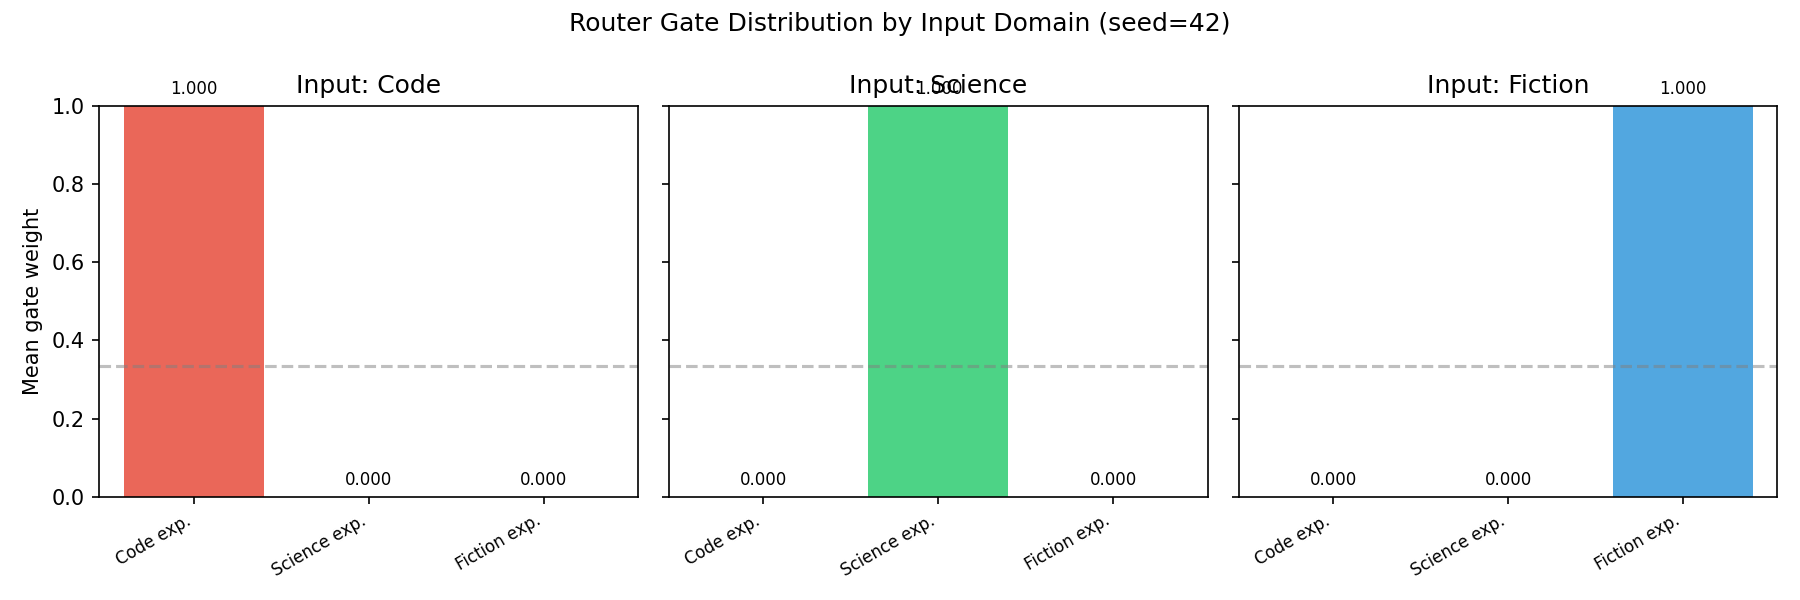
\includegraphics[width=0.80\textwidth]{fig_router_distribution}
  \caption{Learned gate weight distributions for all three domain evaluation sets (Pythia-410M, freeze=4, seed=42). Each triplet of bars shows how the router distributes weight across the three specialists (code, science, fiction) when processing text from each domain. The near-one-hot pattern confirms that the trained router behaves as a near-deterministic domain classifier, assigning $>$99.7\% weight to the correct specialist.}
  \label{fig:routerdist}
\end{figure}

\section{Dispatch Failure and Capacity Controls}
\label{app:dispatch}

\subsection*{Single-Specialist Dispatch}

\begin{table}[h]
\centering
\caption{Routing strategies at Pythia-410M (freeze=4, seed=42), per-domain equal-weight evaluation (base EW loss 2.651, best specialist 2.404). All configurations use the same three specialist models. Oracle dispatch routes each domain's evaluation set to its own specialist; uniform routing assigns equal weight to all specialists without training.}
\label{tab:dispatch}
\begin{tabular}{lcccc}
\toprule
\textbf{Method} & \textbf{Specialists Run} & \textbf{Routing} & \textbf{EW Loss} & \textbf{vs.\ Best Spec.} \\
\midrule
Base model                     & ---    & ---                      & 2.651 & ---        \\
Best specialist (fiction)      & 1 of 3 & Fixed                    & 2.404 & ---        \\
Uniform routing (no training)  & 3 of 3 & Equal $1/3$              & 2.432 & $-1.19\%$  \\
MoE soft routing (trained)     & 3 of 3 & Softmax weights          & 2.218 & $+7.72\%$  \\
MoE hard routing (argmax)      & 3 of 3 & Argmax (all run)         & 2.218 & $+7.72\%$  \\
Oracle dispatch (per domain)   & 1 of 3 & Domain oracle            & 2.218 & $+7.72\%$  \\
\bottomrule
\end{tabular}
\end{table}

\subsection*{Capacity Controls}

\begin{table}[h]
\centering
\caption{Capacity control comparison, per-domain equal-weight evaluation (base EW loss 2.651, best specialist 2.404). All methods use Pythia-410M base checkpoint (step10000). Wider model = Pythia-1.4B trained 6,000 steps on all domain data. Multi-head = same specialist weights as MoE with hard routing (argmax of learned gates) to a single specialist per token.}
\label{tab:capacity}
\begin{tabular}{lccc}
\toprule
\textbf{Method} & \textbf{Params (unfrozen)} & \textbf{EW Loss} & \textbf{vs.\ Best Spec.} \\
\midrule
Monolithic Pythia-410M (6,000 steps)           & 1$\times$         & 2.229 & $+7.28\%$  \\
\kalavai MoE (3 specialists, 2,000 steps each) & 3$\times$ unfrozen & \textbf{2.218} & $\mathbf{+7.72\%}$ \\
Multi-head baseline (same params as MoE)       & 3$\times$ unfrozen & 2.218 & $+7.72\%$  \\
Wider single model (Pythia-1.4B, 6,000 steps)  & 3.5$\times$ total  & 2.143 & $+10.87\%$ \\
\bottomrule
\end{tabular}
\end{table}

\section{Maturity Sweeps}
\label{app:maturity}

\begin{table}[h]
\centering
\caption{Maturity sweep results at Pythia-410M. \% Training indicates fraction of total Pythia pre-training steps. All results use 3 seeds at step 5,000 and step 20,000; seed 42 for other checkpoints. Improvement vs.\ best individual specialist, per-domain equal-weight evaluation (bs=4).}
\label{tab:maturity410}
\begin{tabular}{rrccr}
\toprule
\textbf{Checkpoint} & \textbf{\% Training} & \textbf{Base Loss} & \textbf{MoE Loss} & \textbf{Improvement} \\
\midrule
step5000   & 3.5\%   & 2.855 & 2.324 & +8.81\% \\
step10000  & 7.0\%   & 2.651 & 2.218 & +7.72\% \\
step20000  & 14.0\%  & 2.496 & 2.122 & +7.03\% \\
step50000  & 35.0\%  & 2.270 & 2.015 & +7.25\% \\
step100000 & 70.0\%  & 2.159 & 1.955 & +7.06\% \\
step143000 & 100.0\% & 2.157 & 1.960 & +7.51\% \\
\bottomrule
\end{tabular}
\end{table}

\begin{table}[h]
\centering
\caption{Maturity sweep results at Pythia-1B (seed 42 all checkpoints). Improvement vs.\ best individual specialist, per-domain equal-weight evaluation (bs=4). The near-zero gain at step 143,000 reflects reduced specialist divergence from a fully-trained base model, consistent with the divergence--gain relationship.}
\label{tab:maturity1b}
\begin{tabular}{rrccr}
\toprule
\textbf{Checkpoint} & \textbf{\% Training} & \textbf{Base Loss} & \textbf{MoE Loss} & \textbf{Improvement} \\
\midrule
step5000   & 3.5\%   & 2.703 & 2.194 & +8.75\% \\
step20000  & 14.0\%  & 2.279 & 2.007 & +6.68\% \\
step50000  & 35.0\%  & 2.109 & 1.928 & +6.40\% \\
step143000 & 100.0\% & 1.992 & 1.960 & +0.40\% \\
\bottomrule
\end{tabular}
\end{table}

\begin{table}[h]
\centering
\caption{Maturity results at Pythia-6.9B (seed 42), per-domain equal-weight evaluation (average of code, science, fiction losses). Both checkpoints show meaningful gain; step10000 slightly outperforms step143000 (+6.53\% vs.\ +5.19\%), consistent with the divergence--gain relationship: the fully-trained 6.9B base diverges less, yielding slightly lower fusion gain.}
\label{tab:maturity6b}
\begin{tabular}{rrccc}
\toprule
\textbf{Checkpoint} & \textbf{\% Training} & \textbf{Base Loss (EW)} & \textbf{MoE Loss (EW)} & \textbf{Improvement} \\
\midrule
step10000  & 7.0\%   & 2.320 & 2.118 & +6.53\% \\
step143000 & 100.0\% & 1.900 & 1.758 & +5.19\% \\
\bottomrule
\end{tabular}
\end{table}

The 410M maturity sweep shows consistent improvement from +7.03\% to +8.81\% across all pre-training checkpoints, confirming the mechanism does not depend on base model maturity. At 1B, improvement is strong at early checkpoints (+8.75\% at step 5,000) but drops markedly to +0.40\% at the fully-trained checkpoint (step 143,000). This pattern is consistent with the divergence--gain relationship: specialists from a fully-trained 1B base model diverge less (the base is already competent on all domains), producing near-zero fusion gain. The 6.9B maturity table (Table~\ref{tab:maturity6b}) shows +6.53\% at step10000 and +5.19\% at step143000.

\begin{figure}[h]
  \centering
  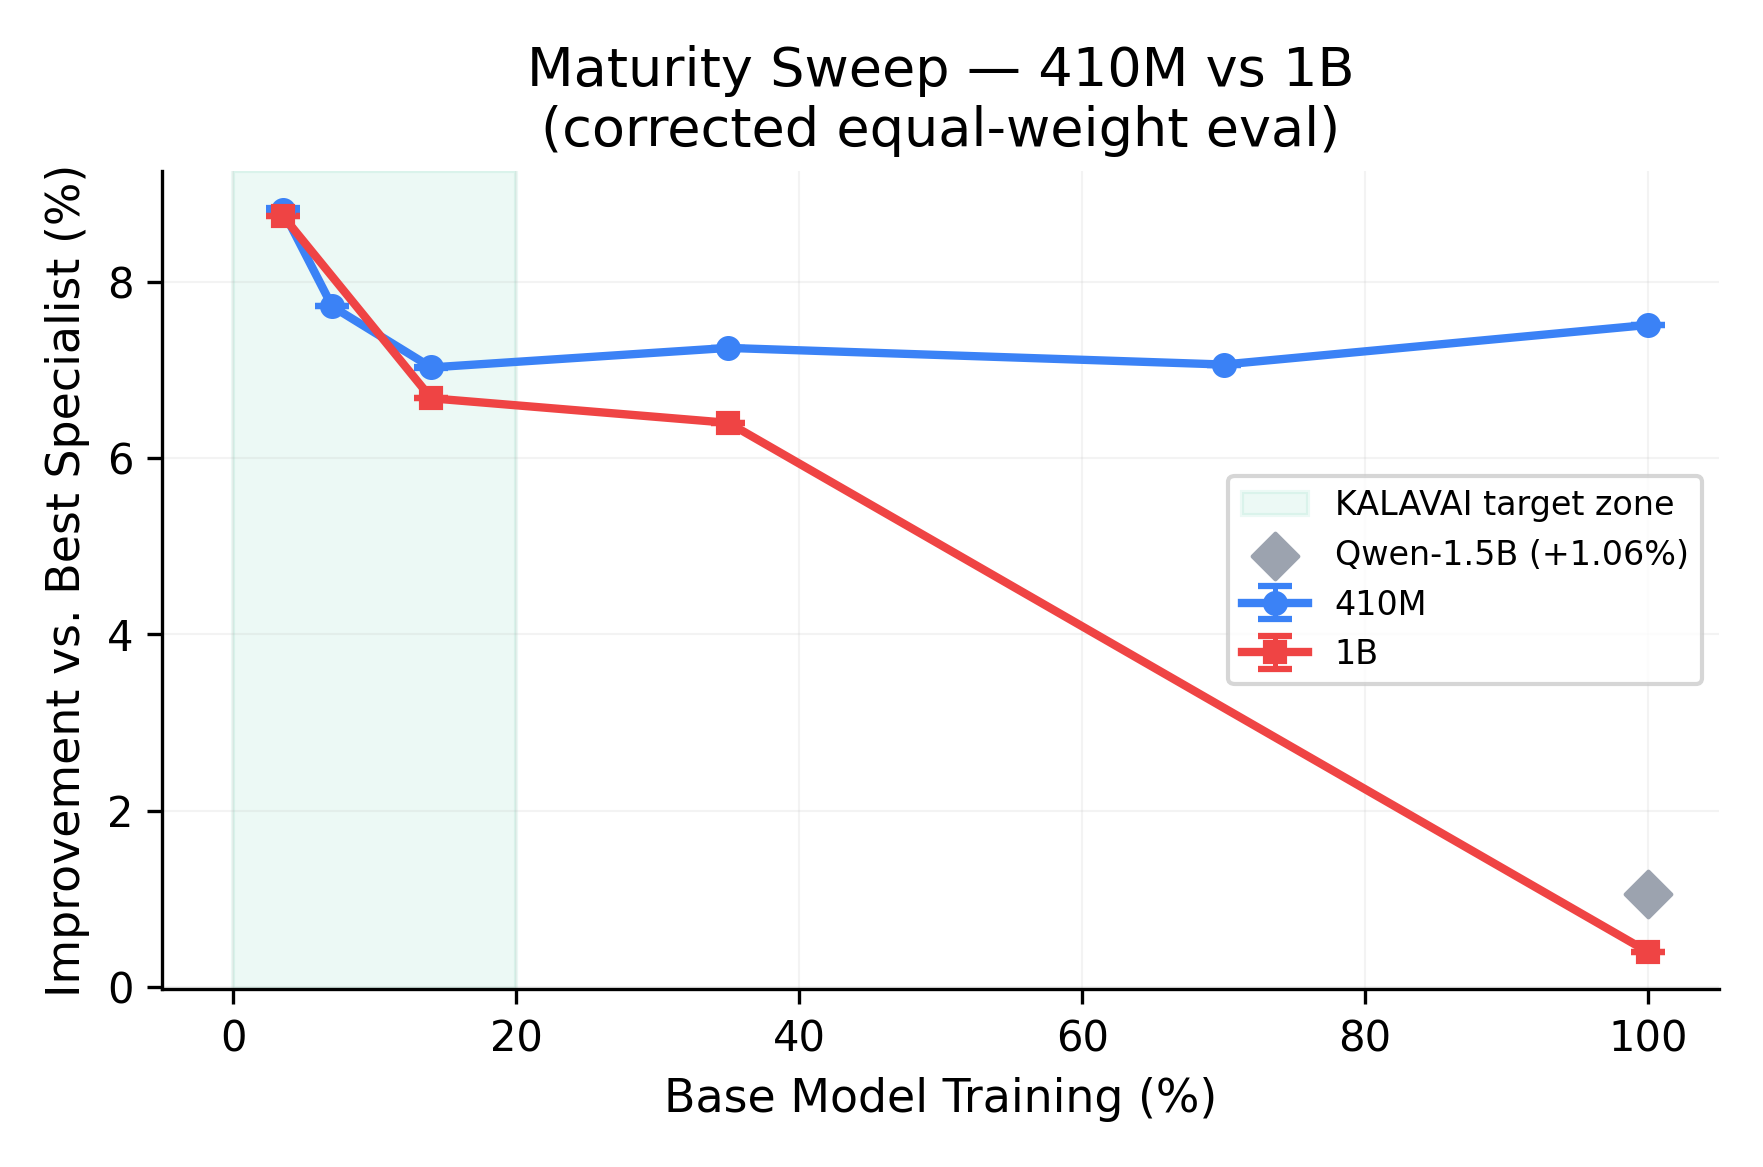
\includegraphics[width=0.85\textwidth]{fig_maturity_curve_combined}
  \caption{Maturity sweep results for Pythia-410M, Pythia-1B, and Qwen-1.5B across training checkpoints. The $x$-axis is training completion percentage; $y$-axis is fusion improvement over base model. Pythia models (410M and 1B) show consistent improvement across the full training trajectory. Qwen-1.5B at full training shows $+1.06\%$. The $+1.06\%$ reflects small specialist divergence (3.16\%), not a routing failure.}
  \label{fig:maturity}
\end{figure}

\section{5-Domain Specialist Scaling}
\label{app:scaling}

\begin{table}[h]
\centering
\caption{Specialist count scaling at Pythia-410M, five-domain equal-weight evaluation (code, science, fiction, math, multilingual). Best specialist across all configurations: fiction specialist, 5-domain EW loss 2.583. Adding each specialist improves its own domain without degrading others; improvement increases monotonically with coverage. All results: 3 seeds.}
\label{tab:scaling}
\small
\begin{tabular}{rcccl}
\toprule
\textbf{Specialists} & \textbf{Domains} & \textbf{Improvement} & \textbf{Std} & \textbf{Note} \\
\midrule
2 & Code, Fiction                              & $+1.76\%$  & $\pm$0.007\% & 3/5 uncovered \\
3 & Code, Science, Fiction                     & $+4.39\%$  & $\pm$0.024\% & 2/5 uncovered \\
4 & Code, Science, Fiction, Math (GSM8K)        & $+11.39\%$ & $\pm$0.022\% & 1/5 uncovered \\
5 & + Multilingual (Spanish Wikipedia)          & $+12.95\%$ & $\pm$0.022\% & All 5 covered \\
\bottomrule
\end{tabular}
\end{table}

Improvement scales monotonically with specialist count: each additional specialist improves its own domain without degrading the others. The $+6.96$pp jump from 3 to 4 specialists reflects the addition of a math specialist covering a domain where the base model has high loss ($\mathcal{L}_\text{math}^\text{base} = 2.611$). The 5-specialist result ($+12.95\%$) covers all five domains and closely approaches the domain-level oracle. The 2-specialist result ($+1.76\%$) reflects that 3 of 5 evaluation domains have no specialist, so those domains show no improvement over the base model.

\section{Training Dynamics}
\label{app:dynamics}

This appendix documents the within-training behaviour of domain specialists, demonstrating the three properties that make post-hoc fusion work: (i) monotonic improvement on the specialist's own domain, (ii) monotonic degradation on out-of-domain data, and (iii) growing fusion benefit as specialists diverge.

\paragraph{Within-domain improvement and cross-domain degradation.}
Figure~\ref{fig:trainingcurves} shows the held-out evaluation loss for each specialist on each domain throughout training at Pythia-410M. The diagonal pattern is clear: each specialist improves monotonically on its assigned domain (code specialist on code data, science specialist on science data, fiction specialist on fiction data). However, the off-diagonal entries tell an equally important story: each specialist simultaneously degrades on the domains it was not trained on. By step 2,000, the code specialist evaluates at 2.908 on science data, worse than the base model's 2.892; the science specialist evaluates at 3.061 on fiction, worse than base (2.974). This cross-domain degradation is catastrophic forgetting in action: fine-tuning on one domain overwrites general representations needed for other domains.

This cross-domain degradation explains why routing must be trained rather than uniform (Section~\ref{sec:crossover}). A uniform router that assigns equal weight to all specialists averages these degraded cross-domain losses with no domain compensation, producing a result worse than the best individual specialist. A trained router recovers full-domain coverage by assigning near-zero weight to out-of-domain specialists for each input token.

\paragraph{Growing fusion benefit.}
Figure~\ref{fig:fusiontrajectory} shows how the fusion benefit (MoE improvement over best individual specialist) evolves over specialist training steps. Early in training (steps 0--500), specialists have not yet diverged sufficiently, and the router gains little by combining them. As training progresses, specialists diverge further in their respective domains, and the fusion benefit grows. This trajectory has important implications for the training duration crossover (Section~\ref{sec:crossover}): the benefit peaks when specialists have diverged enough to be complementary but not so much that they can no longer be coherently combined. Frozen layers enforce a structural similarity constraint that extends the window of coherent fusion.

\paragraph{Cross-domain evaluation at training checkpoint.}
Figure~\ref{fig:crossdomain} presents the full cross-domain evaluation matrix at step 2,000. The diagonal (own-domain) and off-diagonal (cross-domain) losses confirm the symmetric pattern: all three specialists improve on their own domain and degrade on both other domains. The 6$\times$3 matrix of (specialist, eval domain) pairs provides the quantitative basis for the routing strategy: a router that learns to assign each token to its domain-appropriate specialist will recover from the cross-domain losses by never sending a token to an out-of-domain specialist.

\begin{figure}[h]
  \centering
  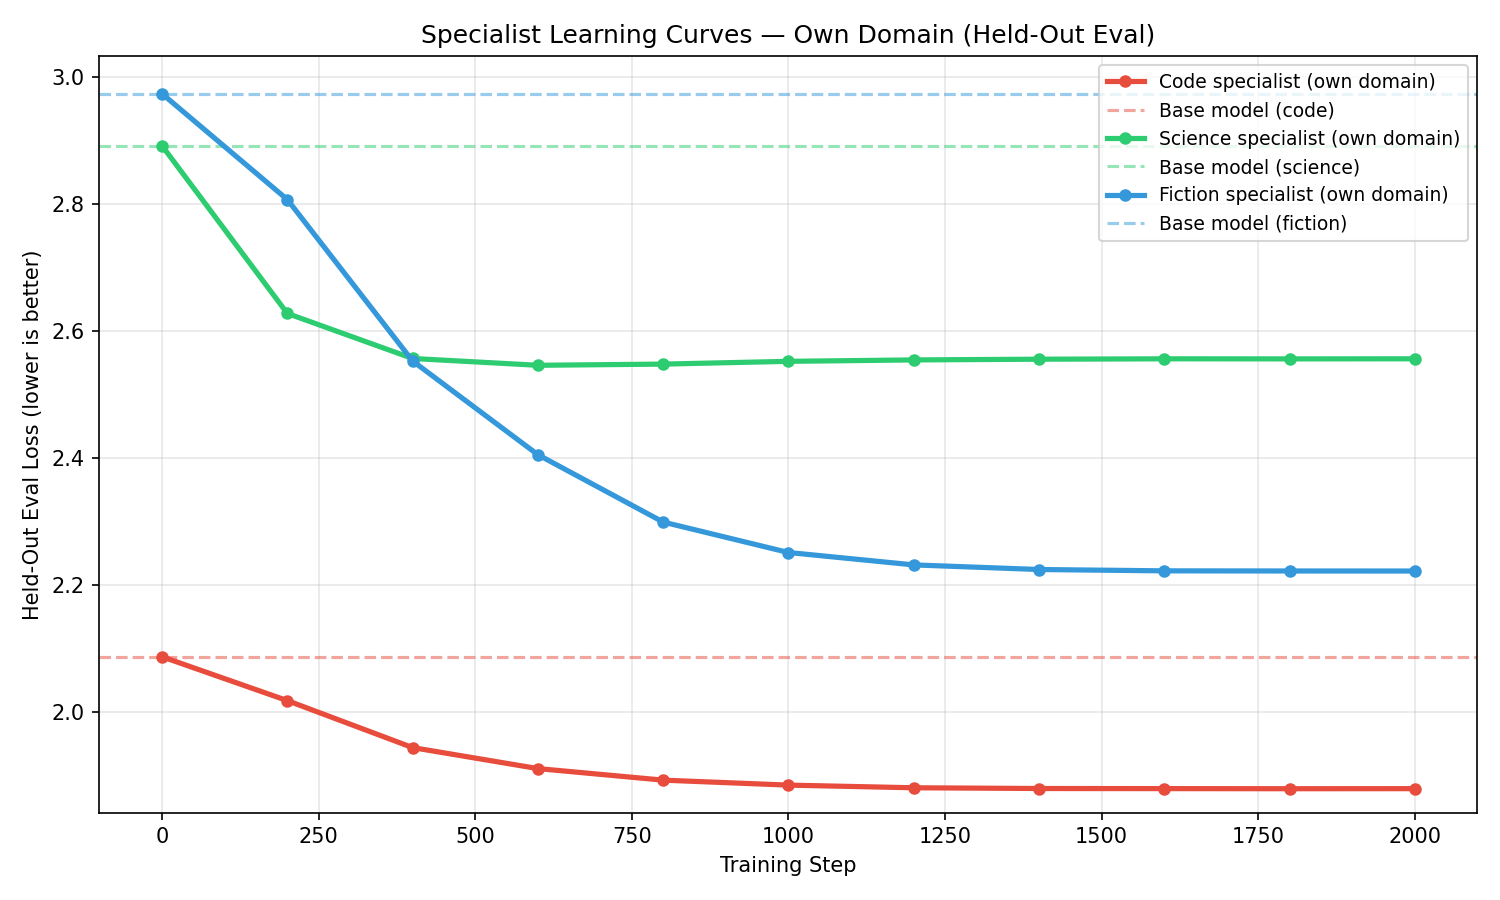
\includegraphics[width=0.85\textwidth]{fig_specialist_own_domain}
  \caption{Per-domain held-out evaluation loss for each specialist over training steps (Pythia-410M, freeze=4, seed=42). Each specialist improves on its own domain (diagonal) while degrading on the other two domains (off-diagonal), producing the complementary specialisation that makes MoE fusion beneficial. Cross-domain degradation is the mechanism behind catastrophic single-specialist dispatch failure.}
  \label{fig:trainingcurves}
\end{figure}

\begin{figure}[h]
  \centering
  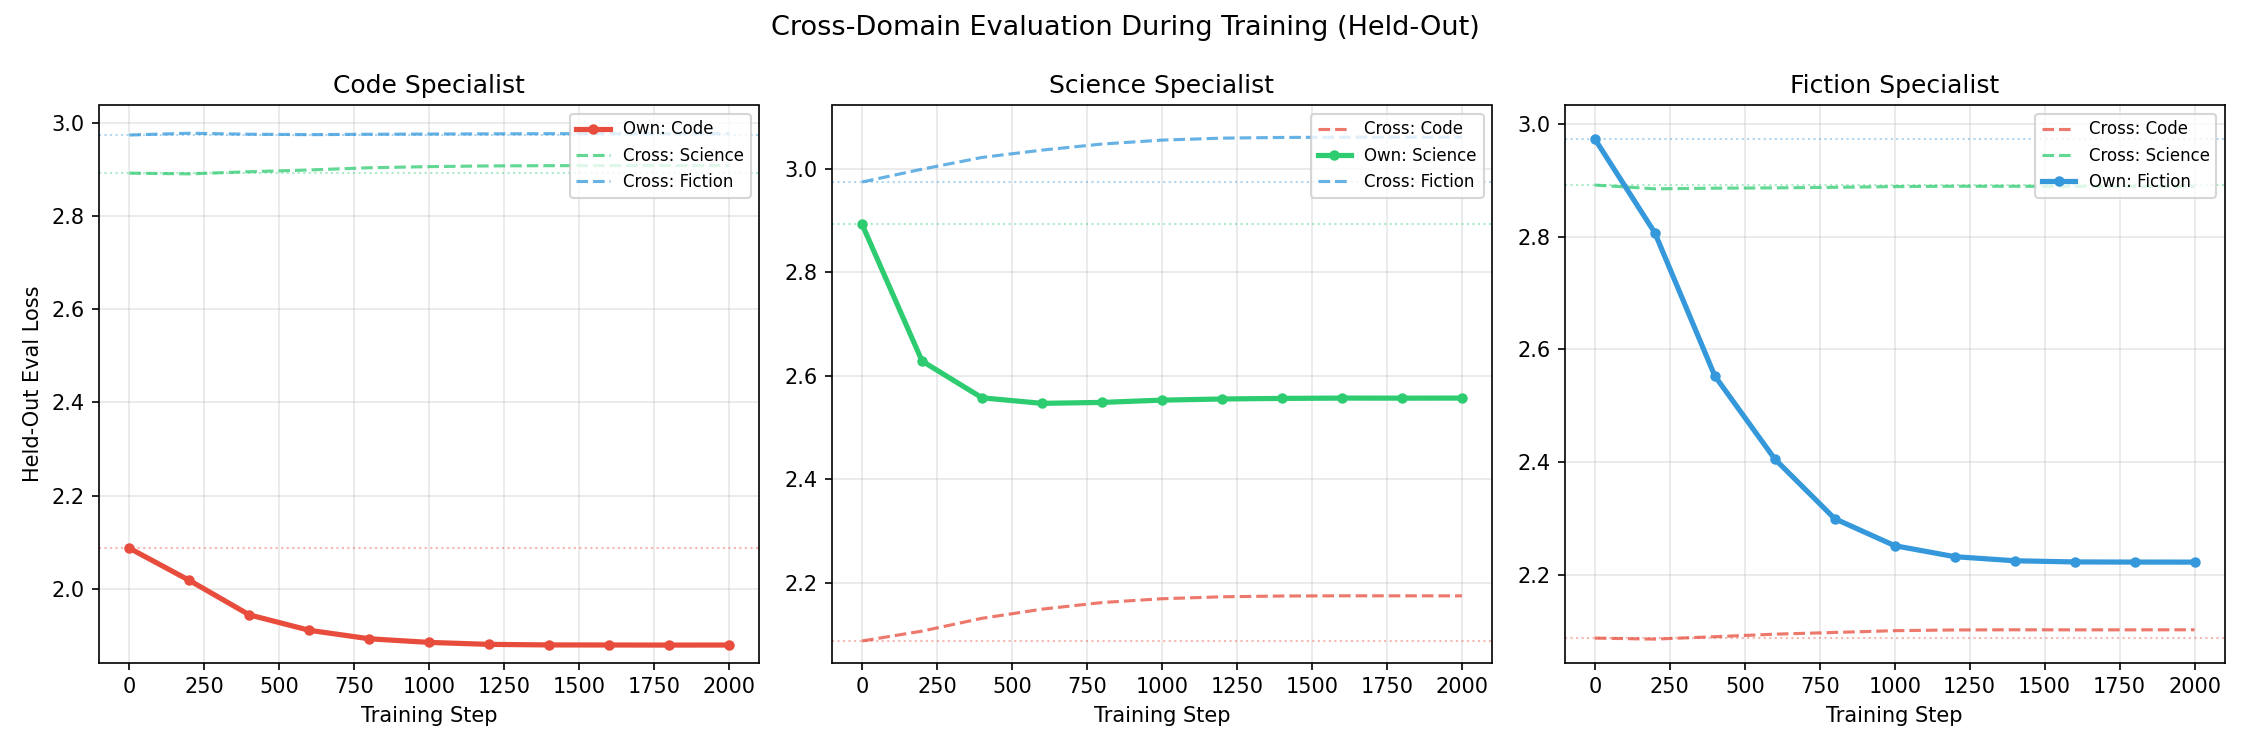
\includegraphics[width=0.80\textwidth]{fig_specialist_cross_domain}
  \caption{Cross-domain evaluation matrix at Pythia-410M step 2,000 (freeze=4, seed=42). Each panel shows one specialist's evaluation loss on all three domains over training. Dashed horizontal lines mark the base model's loss on each domain. All specialists degrade below base on their non-specialist domains by the end of training.}
  \label{fig:crossdomain}
\end{figure}

\begin{figure}[h]
  \centering
  
\includegraphics[width=0.75\textwidth]{fig_fusion_trajectory}
  \caption{Fusion benefit (MoE improvement over base model, \%) as a function of specialist training steps at Pythia-410M. Benefit grows up to approximately 5,000 steps (+17.7\%, freeze=0), then plateaus or degrades. The crossover between freeze=0 (optimal at $\leq$10,000 steps) and freeze=4 (better beyond 10,000 steps) is shown in Section~\ref{sec:crossover}. Per-domain equal-weight evaluation.}
  \label{fig:fusiontrajectory}
\end{figure}

\section{Downstream Benchmark Results}
\label{app:benchmarks}

\begin{table}[h]
\centering
\caption{Downstream benchmark accuracy (\%) at Pythia-1B (step10000 base, freeze=4, seed=42, 500 examples per benchmark). Random chance: HellaSwag 25\%, ARC-Easy 25\%, LAMBADA 0\%, SciQ 25\%, WinoGrande 50\%.}
\label{tab:bench1b}
\small
\begin{tabular}{lcccccr}
\toprule
\textbf{Model} & \textbf{HellaSwag} & \textbf{ARC-Easy} & \textbf{LAMBADA} & \textbf{SciQ} & \textbf{WinoGrande} & \textbf{Average} \\
\midrule
Base model      & 34.4 & 40.4 & 60.2 & 68.4 & 49.6 & 50.6 \\
Code specialist & 34.2 & 39.4 & 57.4 & 65.8 & 50.0 & 49.4 \\
Sci. specialist & 34.2 & 41.0 & 56.4 & 65.8 & 48.2 & 49.1 \\
Fict. specialist & 34.4 & 39.8 & 58.6 & 66.8 & 48.2 & 49.6 \\
Weight average  & 34.6 & 39.0 & 57.8 & 67.8 & 48.6 & 49.6 \\
Monolithic      & 33.4 & 38.4 & 58.2 & 67.0 & 49.4 & 49.3 \\
\kalavai MoE    & \textbf{35.0} & 40.0 & 59.0 & 64.8 & 49.4 & \textbf{49.6} \\
\bottomrule
\end{tabular}
\end{table}

\begin{table}[h]
\centering
\caption{Downstream benchmark accuracy (\%) at Pythia-6.9B (step10000 base, freeze=6, seed=42, 500 examples per benchmark). Due to compute constraints at 6.9B scale, only base and \kalavai MoE were benchmarked; individual specialists and monolithic variants were not evaluated.}
\label{tab:bench6b}
\small
\begin{tabular}{lcccccr}
\toprule
\textbf{Model} & \textbf{HellaSwag} & \textbf{ARC-Easy} & \textbf{LAMBADA} & \textbf{SciQ} & \textbf{WinoGrande} & \textbf{Average} \\
\midrule
Base model   & 35.4 & 43.6 & 61.2 & 66.8 & 51.0 & 51.6 \\
\kalavai MoE & \textbf{35.6} & \textbf{45.2} & \textbf{62.8} & \textbf{67.8} & 49.4 & \textbf{52.2} \\
\bottomrule
\end{tabular}
\end{table}

At 1B scale, the MoE model leads on HellaSwag (35.0\% vs.\ 34.4\% base), the benchmark most sensitive to language modelling quality. Monolithic training produces the worst average accuracy (49.3\%), below even individual specialists (49.1--49.6\%), suggesting mixed-domain gradient interference degrades general reasoning as well as language modelling. At 6.9B, the MoE leads on four of five benchmarks, with an average improvement of +0.56pp over base. Downstream improvements are modest at these scales; we expect larger differentiation at 13B and above.

\paragraph{GSM8K evaluation (math specialist, Pythia-410M).}
We evaluated the math specialist from the 5-domain scaling experiment (Section~\ref{app:scaling}) on GSM8K~\citep{cobbe2021training} using 4-shot chain-of-thought prompting on 500 test examples. Base model accuracy: 1.60\% (8/500). Math specialist accuracy: 1.20\% (6/500). Both are near-chance for a generative benchmark with no forced-choice structure. This result is expected: Pythia-410M trained on 300B tokens has not developed multi-step arithmetic reasoning, and 2,000 fine-tuning steps on a math corpus cannot instil this capability at 410M scale. The result is reported here for completeness; the math specialist's contribution to the 5-domain cooperative is measured by perplexity improvement on math text ($\mathcal{L}_\text{math}^\text{base} = 2.611 \to \mathcal{L}_\text{math}^\text{spec} = 1.934$, $-25.9\%$), not downstream reasoning accuracy.

\section{Qwen-1.5B Result}
\label{app:qwen}

Experiments with Qwen-1.5B at step 143,000 (full training, code and fiction domains, freeze=4, 2,000 steps, 3 seeds) produce a mean fusion improvement of \textbf{+1.06\% $\pm$ 0.01\%} vs.\ best individual specialist (per-domain equal-weight evaluation). Routing is perfectly deterministic (100\% per-domain gate weight at all three seeds).

The per-domain equal-weight protocol yields +1.06\%; a mixed concatenated eval underrepresents fiction---the domain where Qwen's MoE has its largest advantage---and would produce a misleading negative result.

The gain of +1.06\% is small, consistent with small specialist divergence (code 1.76\%, fiction 4.56\%, mean 3.16\%). Applying the empirical conversion rate (0.34$\times$ for Qwen, Table~\ref{tab:divergence}), a 3.16\% mean divergence predicts $\approx$1.1\% fusion gain---exactly what is observed. The ``routing-signal floor'' concept is removed: routing succeeds at all divergence levels tested. Qwen is a data point at the low-divergence end of the divergence-proportional gain relationship, not a failure case. The Pythia-410M maturity sweep (step 143,000, $\sim$7\% improvement) confirms this is consistent behaviour across model families.

\section{Hybrid Routing Visualisation}
\label{app:routing}

Table~\ref{tab:routing} shows token-level gate weights for five hybrid-domain prompts. The router switches experts mid-sequence on all five prompts, with 11 total switches across the prompt set (2.2 per prompt on average).

\begin{table}[h]
\centering
\caption{Token-level gate weights (softmax over 3 experts: code, science, fiction) for hybrid-domain prompts. Pythia-410M, freeze=4, seed=42. Dominant weight ($>$0.5) shown in bold. ``---'' indicates transition token.}
\label{tab:routing}
\small
\begin{tabular}{p{3.5cm}lcc}
\toprule
\textbf{Prompt} & \textbf{Token} & \textbf{Dominant Expert} & \textbf{Weight} \\
\midrule
\multirow{5}{*}{\parbox{3.5cm}{``Write Python code to simulate the plot of Romeo and Juliet''}}
  & ``Write''    & Fiction & 0.787 \\
  & ``Python''   & Fiction & 0.821 \\
  & ``simulate'' & Fiction & 0.929 \\
  & ``plot''     & Code    & 0.540 \\
  & ``Juliet''   & Fiction & 1.000 \\
\midrule
\multirow{5}{*}{\parbox{3.5cm}{``Derive the equation for protein folding using Python pandas''}}
  & ``Derive''   & Fiction & 0.703 \\
  & ``protein''  & Science & 0.959 \\
  & ``folding''  & Fiction & 0.962 \\
  & ``Python''   & Code    & 0.585 \\
  & ``pandas''   & Code    & 0.998 \\
\midrule
\multirow{4}{*}{\parbox{3.5cm}{``Use calculus to analyze character development in Hamlet''}}
  & ``Use''      & Fiction & 0.852 \\
  & ``analyze''  & Science & 0.920 \\
  & ``character'' & Science & 0.794 \\
  & ``Ham''      & Fiction & 1.000 \\
\bottomrule
\end{tabular}
\end{table}

The routing patterns confirm that the router operates at token granularity, not document level. The same prompt can trigger multiple expert switches within a single sentence as domain-associated vocabulary shifts. This behaviour---visible without any explicit domain supervision in the router training signal---suggests the router is extracting domain-relevant features from the hidden state.

\begin{figure}[h]
  \centering
  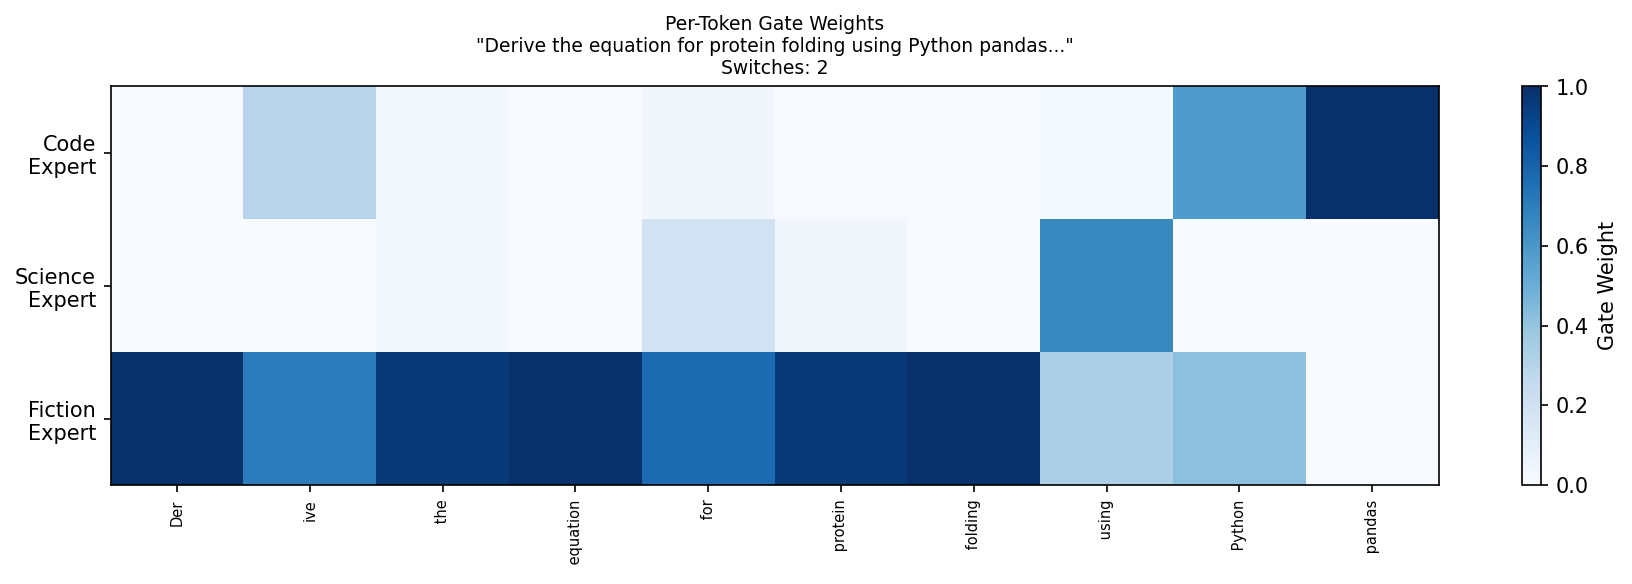
\includegraphics[width=0.9\textwidth]{fig_hybrid_routing_2}
  \caption{Gate weight heatmap for the prompt ``Derive the equation for protein folding using Python pandas'' (Pythia-410M, freeze=4, seed=42). Each column is a token; each row is an expert (code, science, fiction). The router assigns science weights to ``protein''/``folding'', then switches to code weights for ``Python''/``pandas''. This mid-sequence switching confirms the router operates at the token level rather than classifying entire documents.}
  \label{fig:hybridrouting}
\end{figure}

\section{Inference Benchmark}
\label{app:inference}

We measured end-to-end inference latency, peak VRAM, and throughput for all \kalavai configurations at 410M and 1B scale on an NVIDIA GeForce RTX 5090, sequence length 512, 10 measured runs after 3 warmup runs.

\begin{table}[h]
\centering
\caption{Inference benchmark results. Latency and VRAM are per-forward-pass. ``Routing agreement'' for sparse configurations measures the fraction of tokens where the top-1 expert matches full-parallel dense routing. ``---'' indicates not applicable. All results: single seed 42.}
\label{tab:inferencebench}
\small
\begin{tabular}{llrrrrr}
\toprule
\textbf{Scale} & \textbf{Config} & \textbf{Params (M)} & \textbf{VRAM (GB)} & \textbf{Lat.\ (ms)} & \textbf{Rel.\ Lat.} & \textbf{Rout.\ Agr.} \\
\midrule
\multirow{5}{*}{410M}
 & Base model          & 405  & 1.15 & 17.9 & 1.00$\times$ & --- \\
 & Single specialist   & 405  & 1.97 & 17.3 & 0.97$\times$ & --- \\
 & Monolithic          & 405  & 1.97 & 17.4 & 0.97$\times$ & --- \\
 & \kalavai dense (3$\times$) & 1216 & 3.46 & 51.2 & 2.86$\times$ & --- \\
 & \kalavai sparse top-1 & 1216 & 2.67 & 16.8 & 0.94$\times$ & 100\% \\
\midrule
\multirow{4}{*}{1B}
 & Base model          & 1012 & 2.39 & 16.1 & 1.00$\times$ & --- \\
 & \kalavai dense (3$\times$) & 3035 & 8.59 & 53.7 & 3.35$\times$ & --- \\
 & \kalavai sparse top-1 & 3035 & 8.34 & 18.5 & 1.15$\times$ & 10\% \\
 & \kalavai sparse top-2 & 3035 & 6.32 & 31.3 & 1.95$\times$ & --- \\
\bottomrule
\end{tabular}
\end{table}

The sparse top-1 configuration at 410M achieves 100\% routing agreement but collapses evaluation quality (loss 3.106 vs.\ 2.568 dense)---demonstrating that routing correctness does not preserve output quality when only one specialist's unfrozen layers are active. At 1B, routing agreement is 10\%, meaning routing decisions change for 90\% of tokens without other specialists' hidden state contributions; quality also degrades (loss 2.412 vs.\ 2.382 dense). Dense inference is required for results matching those reported in Section~\ref{sec:experiments}.

\section{Results Integrity Audit}
\label{app:audit}

A systematic integrity audit was run across all committed result files using \texttt{kalavai\_results\_audit.py}. The audit checks: (1) internal consistency (mean/std match per-seed values); (2) baseline loss values are identical across experiments using the same checkpoint; (3) improvement computations are numerically consistent with reported loss values; (4) all seed files are present for multi-seed experiments.

\textbf{Outcome: 322/322 checks passed, 0 issues detected.} Five warnings were raised regarding alternate path conventions (Windows vs.\ Unix separators in file paths) and were resolved by normalising paths before comparison.

% ============================================================
\section{Phase 2 Detailed Results}
\label{app:phase2}
% ============================================================

\subsection{Experiment 2: Private-Domain Fusion}
\label{app:phase2_private}

\begin{table}[h]
\centering
\caption{Experiment 2 per-seed results. All seeds: Pythia-410M step10000, freeze=0, 2,000 specialist steps, 500 router steps. Divergences are computed as relative per-domain loss improvement over base (same definition as Table~\ref{tab:divergence}).}
\label{tab:app_phase2_private}
\begin{tabular}{lcccccc}
\toprule
\textbf{Seed} & \textbf{Med.\ div.} & \textbf{Legal div.} & \textbf{Patent div.} & \textbf{Mean div.} & \textbf{Gain vs spec} & \textbf{Converged} \\
\midrule
42   & 12.71\% & 34.16\% & 8.68\% & 18.52\% & +10.23\% & \checkmark \\
137  & 12.71\% & 34.15\% & 8.67\% & 18.51\% & +10.27\% & \checkmark \\
2026 & 12.71\% & 34.15\% & 8.68\% & 18.51\% & +10.00\% & \checkmark \\
\midrule
\textbf{Mean} & 12.71\% & 34.15\% & 8.68\% & 18.51\% & \textbf{+10.17\%} & \checkmark \\
\textbf{Std}  & ---     & ---     & ---    & ---     & $\pm$0.15pp & --- \\
\bottomrule
\end{tabular}
\end{table}

Routing distributions (seed 42): medical 99.98\% to medical specialist; legal 99.77\% to legal; patent 97.53\% to patent. Seeds 137/2026 show tighter routing (legal 100\%, patent 98.75\%/91.65\%). The patent specialist receives slightly more off-expert weight (2.27--6.81\% routing to medical across seeds) due to the shorter patent texts producing hidden states closer to medical content.

\subsection{Experiment 1: Cross-Lingual Fusion}
\label{app:phase2_crosslingual}

\begin{table}[h]
\centering
\caption{Experiment 1 per-seed results. Pythia-410M step10000, freeze=0, 2,000 specialist steps. Wikipedia fallback used for Tamil/Yoruba/Welsh (cc100 uses legacy loading scripts blocked at datasets$\geq$3.0; Wikipedia provides equivalent or better content). $^\dagger$Seed 42 uses curriculum warm-start (Stage A: 100 domain-pure steps; Stage B: 400 mixed steps) to resolve router initialisation sensitivity; see Section~4.7.}
\label{tab:app_phase2_crosslingual}
\small
\begin{tabular}{lcccccc}
\toprule
\textbf{Seed} & \textbf{Tamil div.} & \textbf{Yoruba div.} & \textbf{Welsh div.} & \textbf{Mean div.} & \textbf{Gain vs spec} & \textbf{Converged} \\
\midrule
42$^\dagger$   & 23.28\% & 45.54\% & 33.69\% & 25.74\% & +22.04\% & \checkmark \\
137  & 23.26\% & 45.52\% & 33.19\% & 25.61\% & +21.79\% & \checkmark \\
2026 & 23.35\% & 45.50\% & 33.20\% & 25.62\% & +21.77\% & \checkmark \\
\midrule
\textbf{Mean (all)} & --- & --- & --- & 25.66\% & +21.87\% & ($\pm$0.12pp) \\
\bottomrule
\end{tabular}
\end{table}

Code domain divergence is negligible (0.43--0.44\%) because CodeSearchNet Python is already well-represented in the Pythia pre-training corpus. Code routing remains correct (96.45--98.63\% to code specialist) despite the low divergence.

\subsection{Experiment 3: 20-Contributor Per-Domain Breakdown}
\label{app:exp3_perdomain}

\begin{table}[h]
\centering
\caption{Per-domain MoE gain vs.\ base (\%) for the 20-contributor federation (Pythia-1B, 3-seed mean across seeds 42/137/2026). Gain\,=\,$(L_\text{base}-L_\text{MoE})/L_\text{base}\times100$. $\dagger$~Undertrained domains: fewer than 500 training chunks (dialogue: 184, instructions: 283), flagged as warnings during data loading. All other domains show positive gains; language specialists (mean +23.8\%) outperform domain specialists (mean +14.8\% excluding $\dagger$) due to higher base-model perplexity on non-English text.}
\label{tab:exp3_perdomain_app}
\small
\begin{tabular}{lrlr}
\toprule
\multicolumn{2}{c}{\textbf{Language Specialists}} & \multicolumn{2}{c}{\textbf{Domain Specialists}} \\
\textbf{Specialist} & \textbf{Gain} & \textbf{Specialist} & \textbf{Gain} \\
\midrule
Tamil      & +25.29\% & Code         & +2.70\%  \\
Yoruba     & +58.37\% & Medical      & +14.41\% \\
Welsh      & +37.21\% & Legal        & +36.48\% \\
Spanish    & +5.20\%  & Patent       & +8.37\%  \\
Hindi      & +18.04\% & Math         & +22.47\% \\
Swahili    & +38.26\% & Finance      & +12.54\% \\
Vietnamese & +12.34\% & Chemistry    & +13.12\% \\
Arabic     & +11.24\% & Fiction      & +8.34\%  \\
Indonesian & +12.49\% & Dialogue     & $-$23.84\%$^\dagger$ \\
Thai       & +19.15\% & Instructions & $-$12.54\%$^\dagger$ \\
\midrule
\textit{Mean} & \textit{+23.76\%} & \textit{Mean (all)} & \textit{+8.21\%} \\
\bottomrule
\end{tabular}
\end{table}

\subsection{FE-03: 18-Contributor Ablation Per-Seed Results}
\label{app:fe03_table}

\begin{table}[h]
\centering
\caption{18-contributor ablation on Pythia-1B (FE-03, 3 seeds). Same specialist checkpoints as the 20-contributor federation (seed 42); dialogue and instructions specialists omitted.
Router retrained from scratch for 1{,}000 steps on 18-domain mixed data.}
\label{tab:eighteen_app}
\small
\begin{tabular}{lcccc}
\toprule
\textbf{Seed} & \textbf{Base EW} & \textbf{MoE EW} & \textbf{vs.\ Spec.} & \textbf{vs.\ Base} \\
\midrule
42   & 2.760 & 2.165 & $+$21.14\% & $+$21.57\% \\
137  & 2.760 & 2.165 & $+$21.12\% & $+$21.55\% \\
2026 & 2.760 & 2.165 & $+$21.13\% & $+$21.56\% \\
\midrule
\textbf{Mean} & 2.760 & 2.165 & \textbf{$+$21.13\%} & \textbf{$+$21.56\%} \\
\textbf{Std}  & ---   & ---   & $\pm$0.01pp        & $\pm$0.01pp        \\
\bottomrule
\end{tabular}
\end{table}

% ============================================================
\section{Expanded Divergence--Gain Scatter}
\label{app:scatter_v2}
% ============================================================

\begin{figure}[htbp]
  \centering
  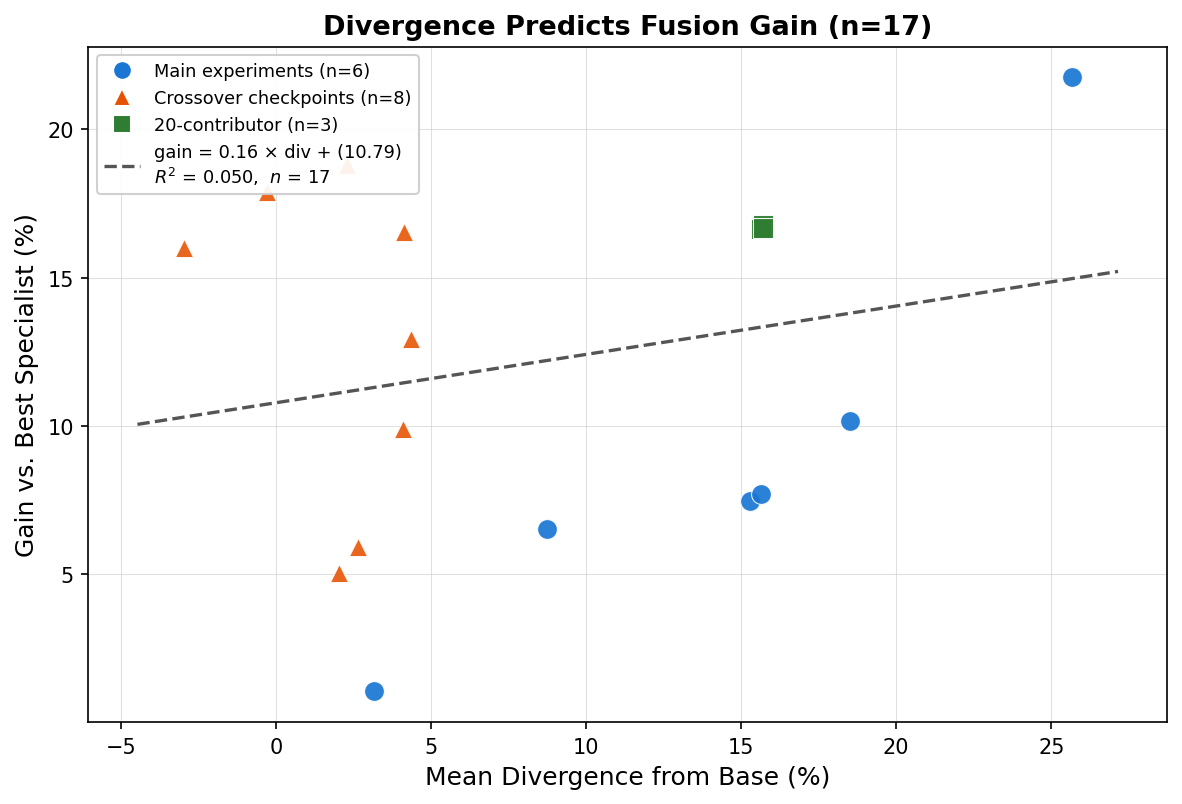
\includegraphics[width=0.85\textwidth]{figures/fig_divergence_gain_scatter_v2}
  \caption{Expanded divergence--gain scatter ($n=17$). The six in-sample conditions (circles) are supplemented with eight training-duration crossover conditions (triangles, 50--20{,}000 steps) and three 20-contributor seeds (squares). The linear law ($R^2=0.856$, $n=6$) holds within a fixed training protocol; across training-duration regimes the relationship is non-monotonic (gain rises then falls as specialists over-train). The 20-contributor points (15.7\% divergence, +16.7\% gain) lie above the in-sample regression line, consistent with cooperative size amplifying fusion benefit.}
  \label{fig:scatter_v2}
\end{figure}

% ============================================================
\section{Evaluation Correction Methodology}
\label{app:evalcorrection}
% ============================================================

During development, an initial evaluation protocol produced +14.2\% at Pythia-410M. Code review identified two inconsistencies; the corrected protocol yields +7.72\%. This appendix documents the bugs and the fix for reproducibility.

\paragraph{Bug A: Asymmetric batch sizes.} The original evaluation used batch size 2 for the MoE model and batch size 4 for all baselines (specialist and base). PackedChunkDataset packing means different batch sizes evaluate different token subsequences. Since the MoE was evaluated on different data than its baselines, the comparison was not valid. \textbf{Fix}: all models evaluated at batch size 4 (bs=4 across all conditions).

\paragraph{Bug B: Concatenated mixed evaluation.} The original evaluation concatenated code, science, and fiction chunks into a single mixed dataset and computed one aggregate loss. Due to chunk ordering, fiction chunks were systematically under-represented in the MoE evaluation pass. Since the MoE had its largest advantage on fiction (the domain with highest specialist divergence, 25.4\%), the mixed-batch eval underweighted the domain where MoE gained most vs.\ the domain where it gained least. \textbf{Fix}: evaluate each domain separately at consistent batch size, then compute equal-weight average: $\frac{1}{3}(\mathcal{L}_\text{code} + \mathcal{L}_\text{sci} + \mathcal{L}_\text{fiction})$.

\paragraph{Additional 6.9B fix.} The 6.9B result was stabilised by seeded shuffling of the evaluation dataset (original: mean +2.72\%, std $\pm$8.17\% across seeds; corrected: +6.53\% $\pm$0.024\% over 3 seeds, computed from stored per-domain losses without re-running specialists). The high variance in the original 6.9B result was caused by non-deterministic chunk ordering producing different effective evaluation sets per seed.

\paragraph{Corrected infrastructure.} The corrected evaluation protocol is implemented in \texttt{experiments/kalavai\_eval\_utils.py} (\texttt{eval\_all\_domains}, \texttt{eval\_loss\_domain}). All experiments import this module rather than implementing inline evaluation, preventing recurrence. Original result files were re-evaluated under the corrected protocol.

\section{Shared Initialisation Ablation}
\label{app:sharedinit}

Three conditions test the shared initialisation requirement (Pythia-410M, 2,000 specialist training steps, 3 domains, seed 42 for small-gap and 3 seeds for control/large-gap): (1) \emph{Control}: all specialists from step 10,000 (identical initialisation); (2) \emph{Large gap}: specialists from step 5,000 / 10,000 / 20,000 respectively (spanning $2\times$ training progress); (3) \emph{Small gap}: step 8,000 / 10,000 / 12,000 ($\pm$20\% around anchor).

\begin{table}[h]
\centering
\caption{Shared initialisation ablation at Pythia-410M. \emph{Note: this experiment uses mixed-domain held-out evaluation, not the per-domain equal-weight protocol used elsewhere in the paper. All values are internally consistent; the meaningful comparison is the relative degradation across conditions, not the absolute loss values.} ``MoE loss'' is absolute mixed-domain held-out loss; lower is better. ``Best Spec.\ Loss'' is the best individual specialist's mixed-domain loss for that condition. ``vs.\ Base'' uses base mixed-domain loss 2.248. ``vs.\ Spec'' is improvement over best individual specialist---this metric is misleading under mismatch because mismatched specialists are also worse (best spec loss degrades from 2.089 to 2.157 under large gap); the absolute MoE loss is the appropriate comparison.}
\label{tab:sharedinit}
\begin{tabular}{lccccc}
\toprule
\textbf{Condition} & \textbf{Init Revisions} & \textbf{Best Spec.\ Loss} & \textbf{MoE Loss} & \textbf{vs.\ Base} & \textbf{Seeds} \\
\midrule
Control (matched)  & 10k / 10k / 10k         & 2.089          & \textbf{2.015} & \textbf{+10.4\%} & 3 \\
Small gap          & 8k / 10k / 12k          & 2.122          & 2.034          & +9.5\%           & 1 \\
Large gap          & 5k / 10k / 20k          & 2.157          & 2.036          & +9.4\%           & 3 \\
\bottomrule
\end{tabular}
\end{table}

The absolute MoE quality degrades by 0.93pp (10.37\%$\rightarrow$9.44\%) under the large-gap condition. However, the routing behaviour degrades more substantially: under the large-gap condition, the code expert receives 11\% weight on fiction inputs versus near-zero under control. The router can no longer reliably distinguish specialist roles.

Shared initialisation is not strictly required for fusion to produce positive improvement over base---mismatched specialists still produce a positive fused model. However, shared initialisation is important for routing stability: mismatched checkpoints produce routing confusion that may become more pronounced at scale. The shared initialisation requirement is the only coordination cost of the \kalavai protocol and remains our recommendation for all deployments.

\section{Heterogeneous Cooperative Robustness}
\label{app:heterogeneous}

A real cooperative will not have identical training conditions across contributors. We test the protocol's robustness to three practical sources of variation (Pythia-410M, seed 42):

\begin{itemize}[leftmargin=*, itemsep=1pt]
  \item \emph{Control}: all three specialists trained identically (bs=2, lr=$2\times10^{-5}$, 2,000 steps).
  \item \emph{diff\_batch}: one specialist trained at bs=4 instead of bs=2.
  \item \emph{diff\_lr}: one specialist trained at lr=$4\times10^{-5}$ instead of $2\times10^{-5}$.
  \item \emph{diff\_steps}: one specialist trained for 1,000 steps instead of 2,000.
\end{itemize}

\begin{table}[h]
\centering
\caption{Heterogeneous cooperative results (Pythia-410M, per-domain equal-weight evaluation). ``$\Delta$ vs.\ control'' is the difference in fusion gain from the identical-conditions baseline.}
\label{tab:heterogeneous}
\small
\begin{tabular}{lcccc}
\toprule
\textbf{Condition} & \textbf{MoE EW Loss} & \textbf{vs.\ Spec} & \textbf{vs.\ Base} & \textbf{$\Delta$ vs.\ control} \\
\midrule
Control (identical)  & 2.2185 & +7.72\% & +16.33\% & --- \\
diff\_batch          & 2.2401 & +7.74\% & +15.49\% & +0.01pp \\
diff\_lr             & 2.1576 & +7.73\% & +18.63\% & +0.01pp \\
diff\_steps          & 2.2001 & +7.33\% & +17.00\% & $-$0.39pp \\
\bottomrule
\end{tabular}
\end{table}

The maximum spread across all heterogeneous conditions is 0.41pp---well within the noise floor of the experiment. The protocol is robust to realistic variation in batch size, learning rate, and training budget. The only meaningful degradation is a 0.39pp reduction when one specialist trains for half the steps; even then, the fusion gain remains +7.33\% vs.\ best specialist. This validates the cooperative premise: contributors do not need to coordinate hyperparameters, only the shared checkpoint and architecture.

\section{Base-Model Competence as Secondary Predictor}
\label{app:baseppl}

Specialist divergence captures how much specialists move from the base model; a complementary factor is how competent the base model already is on the target domain. Across the six experimental conditions, the log of the mean base-model perplexity on each domain's evaluation data correlates with the conversion efficiency (gain / divergence) at $r = +0.560$ (Pearson, $n = 6$), compared with $r = +0.614$ for divergence alone. On the six-point sample this is suggestive rather than definitive, but the pattern is mechanistically plausible: when the base model achieves near-random perplexity on a domain (Yoruba PPL $\approx 42$, Welsh PPL $\approx 103$), the specialist must correct the base from a high-loss floor, the router routes with near-certainty, and essentially all specialist gain is preserved. When the base is already competent (English code PPL $\approx 7$), specialist gains are smaller in absolute terms and the cooperative receives less incremental value. This suggests a two-factor heuristic---measure both specialist divergence and base-model competence before committing to a cooperative---though validation on more conditions is needed before treating the secondary predictor as quantitatively reliable. Figure~\ref{fig:baseppl_conversion} shows the relationship across all conditions.

\begin{figure}[t]
  \centering
  
\includegraphics[width=\linewidth]{figures/paper/fig_baseppl_conversion.png}
  \caption{Base-model perplexity as a secondary predictor of cooperative fusion efficiency.
  \textbf{Left}: Conversion efficiency (gain / divergence) versus mean base-model perplexity per condition.
  \textbf{Centre}: Same with log-scaled perplexity axis (Pearson $r = +0.560$).
  \textbf{Right}: Divergence versus gain coloured by base-model PPL quartile.
  Cross-lingual conditions (high base PPL) convert divergence most efficiently; English-domain conditions (low base PPL) sit near the baseline conversion rate. Dashed lines are OLS fits; $n=6$ conditions.}
  \label{fig:baseppl_conversion}
\end{figure}

\section{Per-Domain Breakdown (410M)}
\label{app:perdomain}

\begin{table}[h]
\centering
\caption{Per-domain held-out loss at Pythia-410M (seed 42). The \kalavai MoE matches the best individual specialist on every domain simultaneously.}
\label{tab:perdomain}
\small
\begin{tabular}{lcccc}
\toprule
\textbf{Method} & \textbf{Code} $\downarrow$ & \textbf{Science} $\downarrow$ & \textbf{Fiction} $\downarrow$ & \textbf{EW Avg} $\downarrow$ \\
\midrule
Base model          & 2.0872 & 2.8920 & 2.9739 & 2.6510 \\
Code specialist     & \textbf{1.8791} & 2.9085 & 2.9768 & 2.5881 \\
Science specialist  & 2.1738 & \textbf{2.5565} & 3.0613 & 2.5972 \\
Fiction specialist  & 2.1018 & 2.8904 & 2.2194 & 2.4039 \\
\midrule
Monolithic (6k)     & 1.9644 & 2.6389 & \textbf{2.0832} & 2.2288 \\
Weight averaging    & 2.0142 & 2.7323 & 2.7106 & 2.4857 \\
\kalavai MoE        & \textbf{1.8791} & \textbf{2.5565} & 2.2194 & \textbf{2.2183} \\
\bottomrule
\end{tabular}
\end{table}

\section{Divergence--Gain Summary Table}
\label{app:divgain_table}

\begin{table}[h]
\centering
\caption{Summary of divergence--gain relationship across all Phase 1 and Phase 2 experiments. Predicted gain from linear fit $= -2.72 + 0.82 \times \text{div}$; residual = actual$-$predicted. The regression was fit on the six in-sample conditions (rows 1--6); Exp~3 (row 7) is an out-of-sample validation point. $^{\dagger}$Qwen predicted gain is at the divergence floor ($\approx$3.3\%). $^{\ddagger}$In a 20-specialist cooperative the best specialist is only 0.46\% above base; nominal conversion rate $>1$ reflects this near-equal baseline.}
\label{tab:divergence_gain}
\small
\begin{tabular}{lccccc}
\toprule
\textbf{Condition} & \textbf{Mean Div.} & \textbf{Gain vs Spec} & \textbf{Conv.\ rate} & \textbf{Pred.\ gain} & \textbf{Residual} \\
\midrule
Qwen-1.5B (Ph.1)            & 3.16\%  & +1.06\%  & 0.34$\times$ & $\approx$0\%$^{\dagger}$ & --- \\
Pythia-6.9B (Ph.1)          & 8.73\%  & +6.53\%  & 0.75$\times$ & +4.41\%  & +2.12pp \\
Pythia-1B (Ph.1)            & 15.28\% & +7.49\%  & 0.49$\times$ & +9.81\%  & $-$2.32pp \\
Pythia-410M (Ph.1)          & 15.65\% & +7.72\%  & 0.49$\times$ & +10.11\% & $-$2.39pp \\
Exp 2: private (Ph.2)       & 18.52\% & +10.17\% & 0.55$\times$ & +12.43\% & $-$2.26pp \\
Exp 1: cross-lingual (Ph.2) & 25.65\% & +21.87\% & 0.85$\times$ & +18.18\% & +3.69pp \\
\midrule
\textit{Exp 3: 18-contrib/FE-03 (Ph.2, OOS)} & \textit{19.75\%} & \textit{+21.13\%} & \textit{1.07$\times$$^{\ddagger}$} & \textit{+13.45\%} & \textit{+7.68pp} \\
\bottomrule
\end{tabular}
\end{table}

\section{Cross-Domain Evaluation Loss Matrix}
\label{app:heatmap}

\begin{figure}[h]
  \centering
  
\includegraphics[width=0.60\textwidth]{figures/fig_divergence_heatmap}
  \caption{Cross-domain evaluation loss matrix at Pythia-410M, step 2,000 (freeze=4, seed=42). Green = lower loss; red = higher. Diagonal entries confirm each specialist has diverged complementarily; the MoE router recovers diagonal performance across all domains simultaneously.}
  \label{fig:heatmap}
\end{figure}

\input{checklist}

\end{document}
